% !TeX root = ../thesis.tex
\chapter{Grundlagen}
\label{chap:fundamentals_related-work}
In diesem Kapitel werden die Grundlagen eines neuartigen Übertragungssystems vorgestellt. Da eine Audioübertragung mittels \gls{acr:VLC}-Technik implementiert werden soll, wird zunächst auf die Eigenschaften eines zu übertragenden Audiosignals eingegangen. Darauf folgend werden einige Grundlagen zur Übertragungstechnik und der verwendeten elektronischen Bauteile erläutert. Zuletzt setzt sich dieses Kapitel mit Programmen auseinander, welche signifikant für die Realisierung der Übertragung sind. Hier werden grundlegende Funktionsweisen sowie deren Rolle in der analogen und digitalen Signalverarbeitung thematisiert. 

\section{Audio}
\label{subsec:Unterabschnitt1}

Ziel der vorliegenden Abschlussarbeit ist die Übertragung eines Echtzeit-Audio-Signals mithilfe des projektierten \gls{acr:VLC}-Senders. Deshalb soll im nachfolgenden Kapitel anfänglich im Allgemeinen auf die Übertragung von Audiosignalen eingegangen werden. Praktische Beispiele zu der Übertragung von Audiosignalen über größere Entfernung ergeben sich bei der Übertragung von Sprache und Musik. Hierbei wird zunächst der Hörschall mit Hilfe eines Mikrofons in ein proportionales elektrisches Signal umgewandelt. Dieses Signal wird anschließend auf drahtlosem  Wege dem Empfänger übermittelt. Gängige Beispiele für die drahtlose Übertragung sind \gls{acr:WLAN} und der klassische Rundfunk. Am Empfangsort wird das elektrische Signal mittels eines Lautsprechers wieder in ein akustisches Signal umgesetzt.\cite{plassmannHandbuchElektrotechnik2016} Der Lautsprecher erzeugt eine mechanische Welle, die in Hörschall resultiert. Hierbei definiert die Frequenz eine Tonlage und die Amplitude, in diesem Fall, die Lautstärke des Audiosignals. Beim Auftreffen dieser mechanischen Welle auf das menschliche Trommelfell wird dieses in Schwingung versetzt und regt somit die menschlichen Nerven an. Das Signal wird im Ohr von einer mechanischen Welle in ein elektrisches Signal umgewandelt, das über die Nervenbahnen zum Gehirn gelangt. Im Gehirn wird das elektrische Signal verarbeitet und mit semantischen Informationen verbunden. Diese ermöglichen das menschliche Hören.\cite{stotzaudio} Die Wahrnehmung von Tönen bei Menschen hängt jedoch nicht nur von der Amplitude und der Frequenz des Tones ab, sondern auch von der wahrnehmenden Person selbst. Demnach können Menschen nur Töne in einem bestimmten Frequenzbereich wahrnehmen. Frequenzen unterhalb des menschlichen Hörbereichs werden Infraschall genannt, darüber liegende Frequenzen werden als Ultraschall bezeichnet. Dieser Frequenzbereich ist nicht nur von Mensch zu Mensch unterschiedlich, sondern variiert auch mit zunehmendem Alter. Daher kann der Frequenzbereich des menschlichen Hörens nicht pauschal vereinheitlicht werden. Plassmann bringt den Hörbereich zwischen 16 Hz und 16 kHz vor \cite{plassmannHandbuchElektrotechnik2016}, wohingegen Michels ihn zwischen 16 Hz bis 20 kHz ansiedelt \cite{michelsSonographieOrganUnd2012}. Der hörbare Frequenzbereich variiert auch von Lebewesen zu Lebewesen. Hunde haben zum Beispiel ein erheblich feineres Hörorgan als Menschen. Ihr Frequenzbereich erstreckt sich als Folge dessen von 65 Hz bis 45 kHz.\cite{michelsSonographieOrganUnd2012}

\begin{figure}[H]
	\centering
	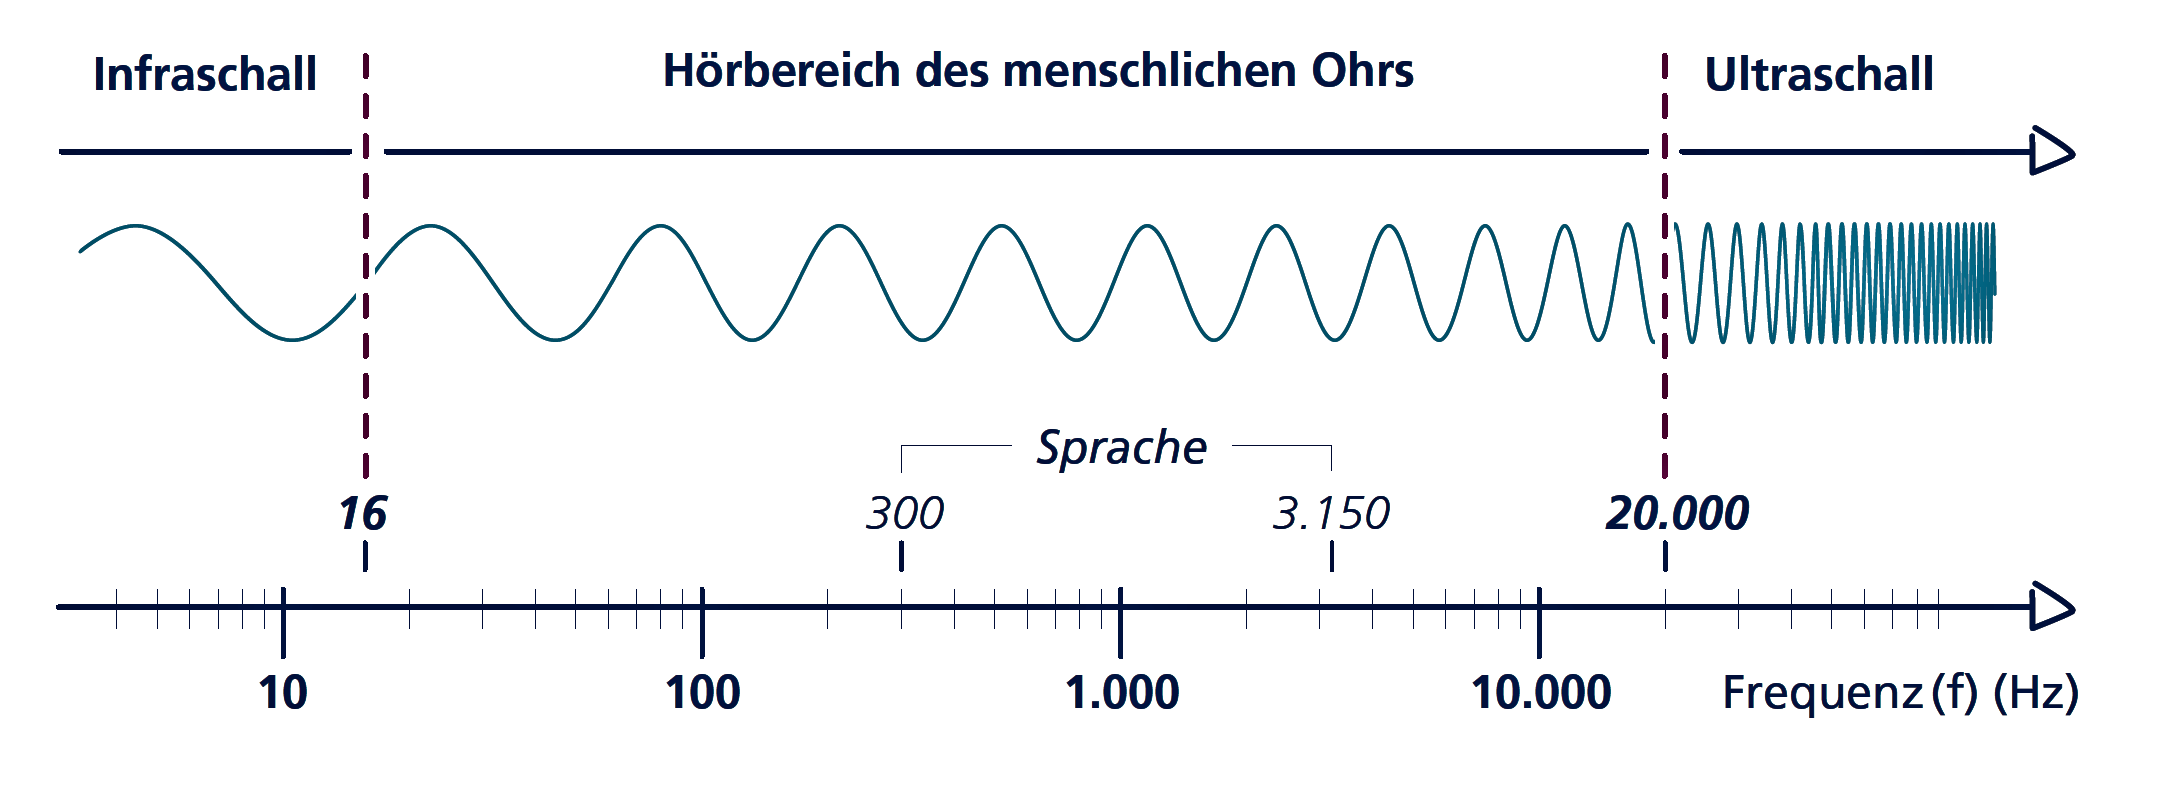
\includegraphics[width=1\textwidth]{audiospektrum.png}
	\caption[Hörbereich des menschlichen Ohres]{Hörbereich des menschlichen Ohres} \cite{michelsSonographieOrganUnd2012}
	\label{fig:audiospektrum}
\end{figure}

Außerdem verändert der Abstand zu einer Quelle zusätzlich die Wahrnehmung des Signals. Die Amplitude einer sich ausbreitenden Welle verringert sich mit zunehmender Distanz, wodurch die Lautstärke abnimmt. Befindet sich eine Quelle außerhalb der Hörreichweite können diese durch analoge oder digitale Kommunikationssysteme abgefangen werden, um eine Übertragung zu ermöglichen. Zur Übertragung und Weiterverarbeitung der beschriebenen mechanischen Welle muss diese zunächst in eine elektrische Größe verwandelt werden. Bei dieser Wandlung wird für Audiosignale ein Mikrofon verwendet. Ähnlich wie es mit dem Trommelfell im menschlichen Ohr passiert, wird im Inneren des Mikrofons eine Membran in Schwingung versetzt und erzeugt dadurch eine elektrische analoge Spannung.
Zur digitalen Verarbeitung des Signals muss dieses mithilfe eines Analog-Digital-Wandlers
(AD-Wandler) in digitale Werte verwandelt werden. Hierfür wird die Analogspannung in zeitlich äquidistanten Abständen ausgewertet und abgespeichert. Es wird also ein Signal mit einem Dirac-Kamm gefaltet um dessen Werte zu ermitteln. Dieser Vorgang wird Abtastung genannt und in Darstellung~\ref{fig:abtastung} illustriert. Diese Abtastung spiegelt einzelne Impulse mit Werten des Signals zu den Abtastzeitpunkten wider. Zwischen den Abtastzeitpunkten wird jedoch keine Information abgefragt, wodurch der Wert an diesen Stellen Null beträgt. Zur Rekonstruierung des Originalsignals müssen durch einen Digital-Analog-Wandler die fehlenden Signalabschnitte interpoliert werden. Um also eine aussagekräftige Abtastung durchzuführen, ist die Korrelation zwischen Abtastfrequenz und Signalfrequenz zu berücksichtigen.


\begin{figure}[H]
	\centering
	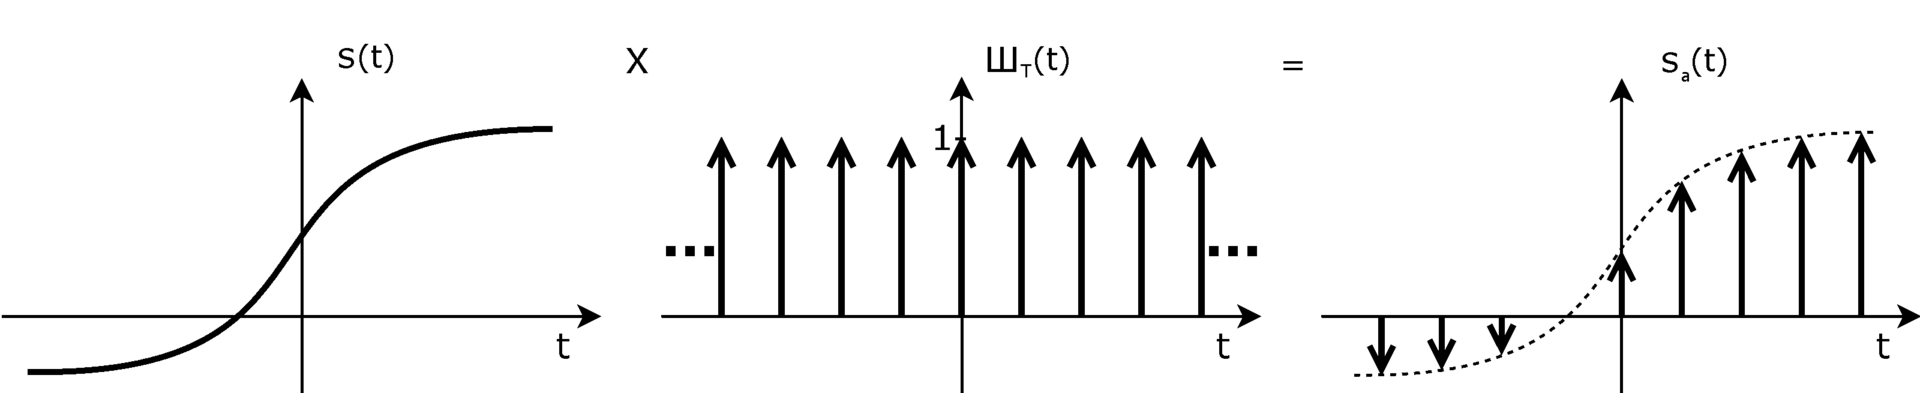
\includegraphics[width=1\textwidth]{abtastung.png}
	\caption[Abtastung eines Signals]{Abtastung eines Signals} \gls{online:abtastung}
	\label{fig:abtastung}
\end{figure}

In Abbildung~\ref{fig:abtastung} ist zu erkennen, dass genügend Abtastwerte vorhanden sind, weshalb der Verlauf des Signals im Nachgang detailliert wiedergegeben werden kann. Abtastfrequenz und Signalfrequenz stehen demnach in einem adäquaten Verhältnis zueinander. Je weniger Abtastwerte vorhanden sind, desto größer werden Messabstände. Dies hat zur Folge, dass eine Rekonstruktion des Signales bald nicht mehr möglich ist.\cite{masteraudio}

Das Abtasttheorem von Shannon besagt, dass für die höchste Signalfrequenz pro Schwingung mindestens zwei mal abgetastet werden muss, um das Signal ausreichend rekonstruieren zu können. Hierbei wird also Formel~\ref{equ:abtast} angewendet.

\begin{equation}
	\label{equ:abtast}
	F_{A} \geq 2 \cdot F_{S}
\end{equation}

Die Variable $F_{A}$ bildet hierbei die Abtastfrequenz ab und $F_{S}$ steht für die höchste im Signal enthaltende Frequenz. In Abbildung~\ref{fig:shannon} wird bei der oberen Abtastung die Regel von Shannon befolgt, wohingegen sie im unteren Teil der Abbildung verletzt wird. An diesem Beispiel ist gut zu erkennen, dass durch die richtige Abtastung eine relativ originalgetreue Rekonstruktion stattfinden kann, während bei einer Unterabtastung das Signal merklich verfälscht rekonstruiert wird. Zuzüglich ist an dieser Darstellung jedoch zu sehen, dass die Abtastung nur den minimalen und den maximalen Wert des Signals abgetastet hat. Dies bedeutet, dass bei einer Phasenverschiebung von $90^\circ$ nur Nulldurchgänge des Signals abgetastet geworden sind, was eine Rekonstruktion unmöglich gemacht hätte. 

\begin{figure}[H]
	\centering
	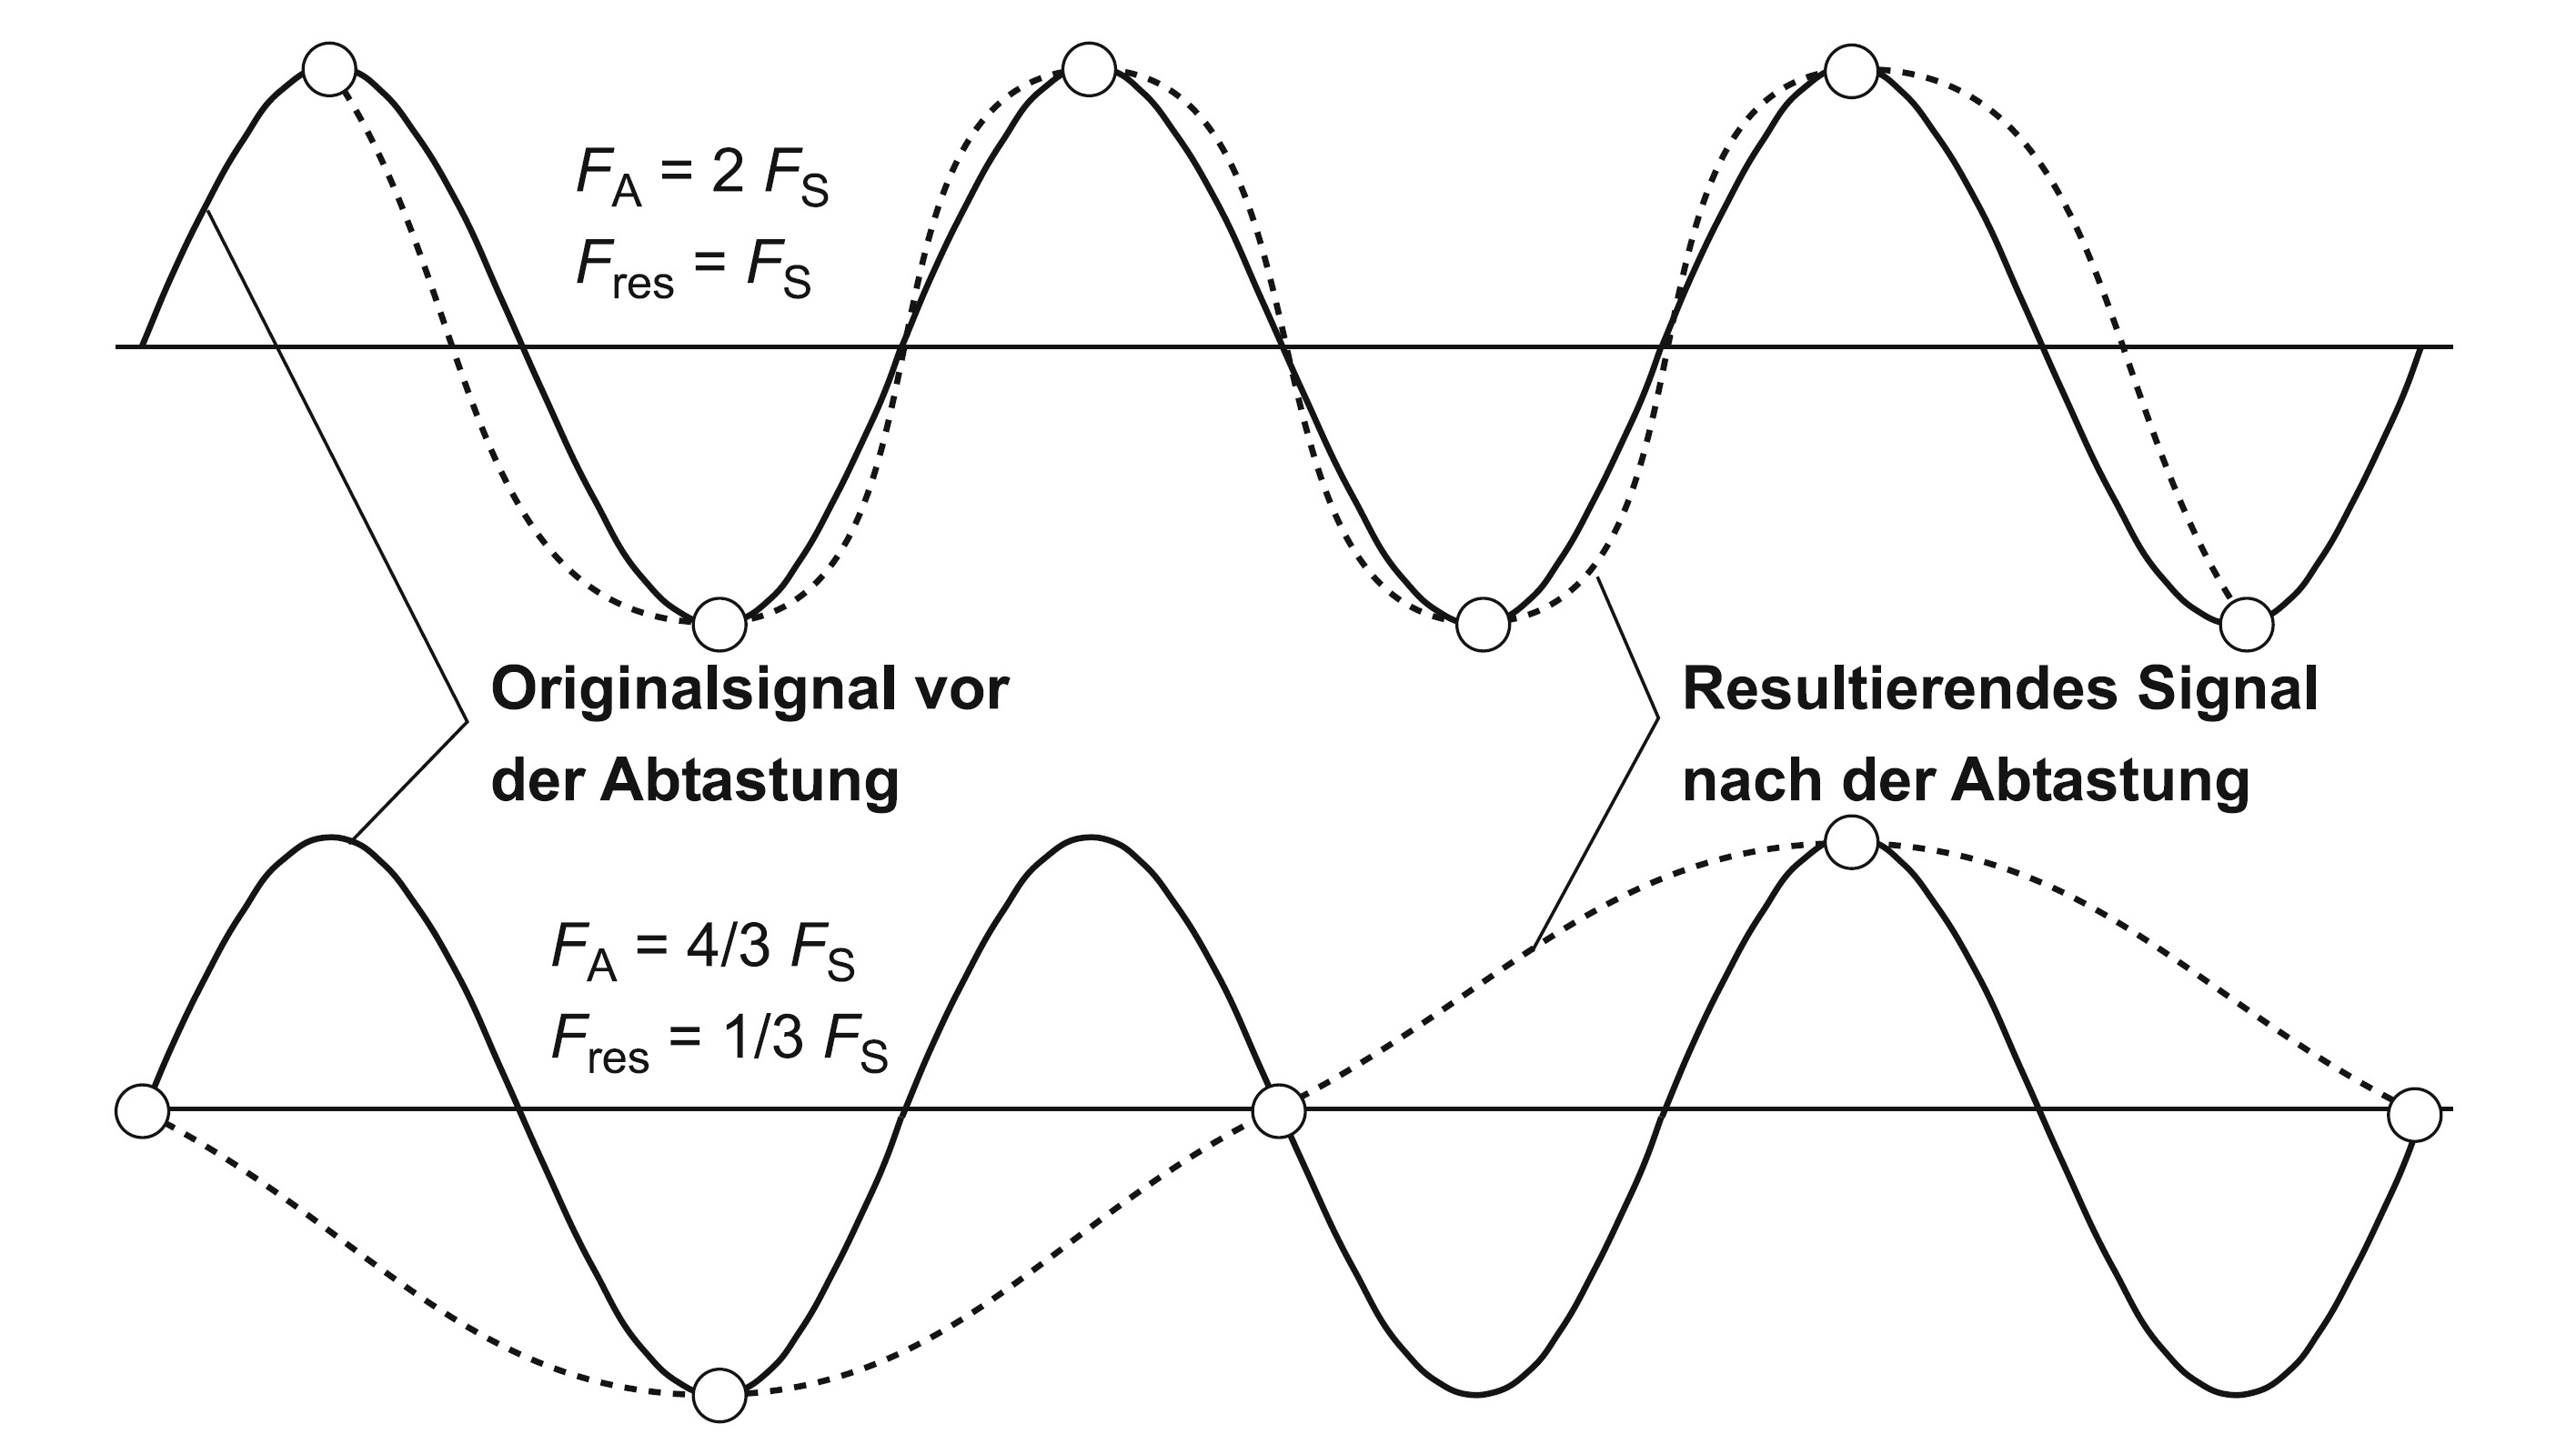
\includegraphics[width=0.8 \textwidth]{shannon.jpg}
	\caption[Vergleich zwischen Abtastung und Unterabtastung eines Signals]{Vergleich zwischen Abtastung und Unterabtastung eines Signals} \cite{stotzaudio}
	\label{fig:shannon}
\end{figure}

Empfehlenswert ist es also, das Shannon Theorem nur als absolute Untergrenze zu wählen und dazu zu neigen die Abtastfrequenz noch deutlich höher als das maximale zu messende Signal zu bestimmen.\cite{stotzaudio} Im Audiobereich wird häufig mit 44,1 kHz oder mit 48 kHz abgetastet und somit das Shannon-Theorem eingehalten, da der Hörbereich des menschlichen Ohrs ~\ref{fig:audiospektrum} bei 20 kHz endet. \cite{masteraudio}


\section{Einführung in die Übertagungstechnik}
\label{subsec:uebertragung}
In diesem Kapitel werden die Grundlagen der modernen Übertragungstechnik als Basis für die weiteren Ausführungen erklärt. Zunächst soll der generelle Aufbau eines Übertragungssystems erläutert werden, um anschließend einige gängige digitale Modulationsarten vorzustellen. Hierbei liegt der Fokus besonders auf der \gls{acr:QAM}-Modulation, welche in der später diskutierten Dream-Software Verwendung findet. Der letzte Abschnitt beschäftigt sich mit den Themen der Bandbreitennutzung und des Mehrkanalzugriffs. Hier werden die aus der Mobilfunktechnik bekannten Begriffe \gls{acr:FDMA}, \gls{acr:TDMA} und \gls{acr:CDMA} eingeführt und beschrieben.

\subsection{Übertragungssystem}
\label{subsec:aufbauueber}

Ein Übertragungssystem ergibt sich vereinfacht dargestellt aus fünf verschiedenen Komponenten. In Abbildung~\ref{fig:komsystem} ist eine Skizze eines solchen Übertragungssystems zu sehen. Zunächst ist eine Quelle vonnöten, welche ein zeitkontinuierliches Signal (z.B. Sprache, Musik, Bilddaten, analoge Messwerte) oder ein zeitdiskretes Signal (z.B. Buchstaben, Datensequenzen, abgetastete analoge Signale) zur Verfügung stellt. Die Informationsquelle (information source) übergibt die Nachricht (message) dem Sender (transmitter). Der Sender übernimmt im System die Aufgabe, die Informationsquelle in ein für die Übertragung geeignetes Format umzuwandeln. Dieses muss auf den später zur Weiterleitung des Signals genutzten Kanal abgestimmt werden, welcher dann das entsprechende Sendesignal (signal) für den Kanal (channel) generiert. Im Kanal addiert sich das Signal der Störquelle (noise source) hinzu, sodass sich das Empfangssignal (received signal) am Empfänger (receiver) ergibt. Dabei gilt es darauf zu achten, den zur Verfügung stehenden Kanal und seine Eigenschaften möglichst effizient zu nutzen und die Störquelle zu minimieren. Sendekanäle sind physikalischer Natur und allgemein fehlerbehaftet. Es wird zwischen drahtlosen Kanälen (elektromagnetisch, akustisch, Infrarot) und drahtgebundenen Kanälen (Kupferleitungen, Glasfaserkabel) unterschieden. Im Anschluss generiert der Empfänger daraus dann die empfangene Nachricht (received message) und leitet jene schließlich der Informationssenke (destination) weiter. In Anbetracht ihrer Anwendung werden diese einzelnen Blöcke des Kommunikationsmodells in weitere Komponenten zerlegt und somit weiter spezialisiert. \cite{wernerNachrichtentechnikEinfuehrungFuer2010}

\begin{figure}[H]
	\centering
	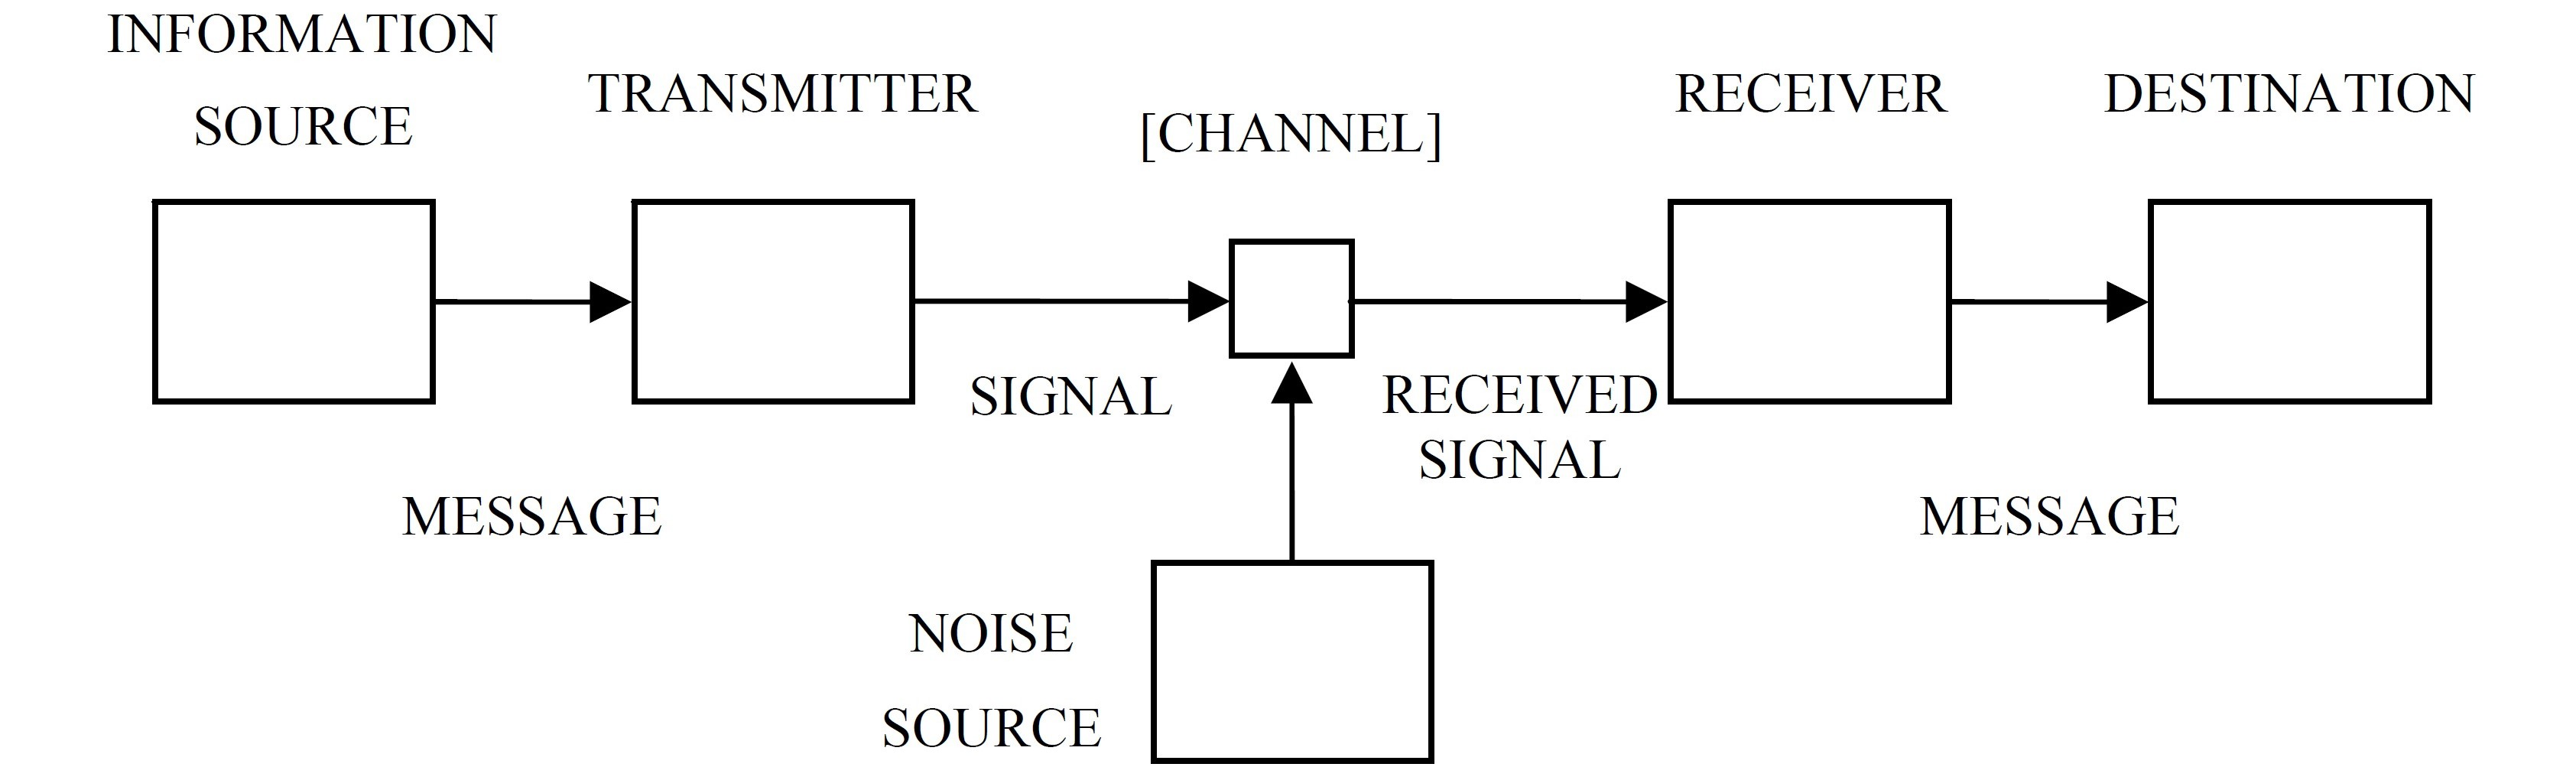
\includegraphics[width=1\textwidth]{komsystem.jpg}
	\caption[Nachrichtenübertragung nach Shannon]{Nachrichtenübertragung nach Shannon} 
	\cite{shannon}
	\label{fig:komsystem}
\end{figure}

Aufgrund der Thematik dieser Abschlussarbeit soll das Augenmerk nun auf ein drahtloses Übertragungssystem gelegt werden. Zur Projektierung eines solchen müssen zunächst der physikalische Kanal und die Signalform festgelegt werden.
So verwenden Fernbedienungen beispielsweise als Signalform Licht im Infrarot-Bereich, um Datenbefehle zu übertragen. Nach einem ähnlichen Prinzip funktioniert auch \gls{acr:VLC}. Die Schwierigkeit ist jedoch, dass der direkte Einfall des Lichts auf den Empfänger gegeben sein muss, weshalb die Reichweite dieser Form der Datenübertragung äußerst begrenzt ist. Daher eignet sie sich beispielsweise nicht für den Mobilfunk. Hier werden üblicherweise elektromagnetische Wellen in Megahertz bis Gigahertz Frequenzbereichen appliziert. Diese Wellen bestehen aus einem magnetischen Feld ($\vec{B}$) und einem elektrischen Feld ($\vec{E}$). Zudem breiten sich jene Felder orthogonal zueinander aus, wie in Abbildung ~\ref{fig:elektromag} veranschaulicht wird.\gls{online:elektromag} 

\begin{figure}[H]
	\centering
	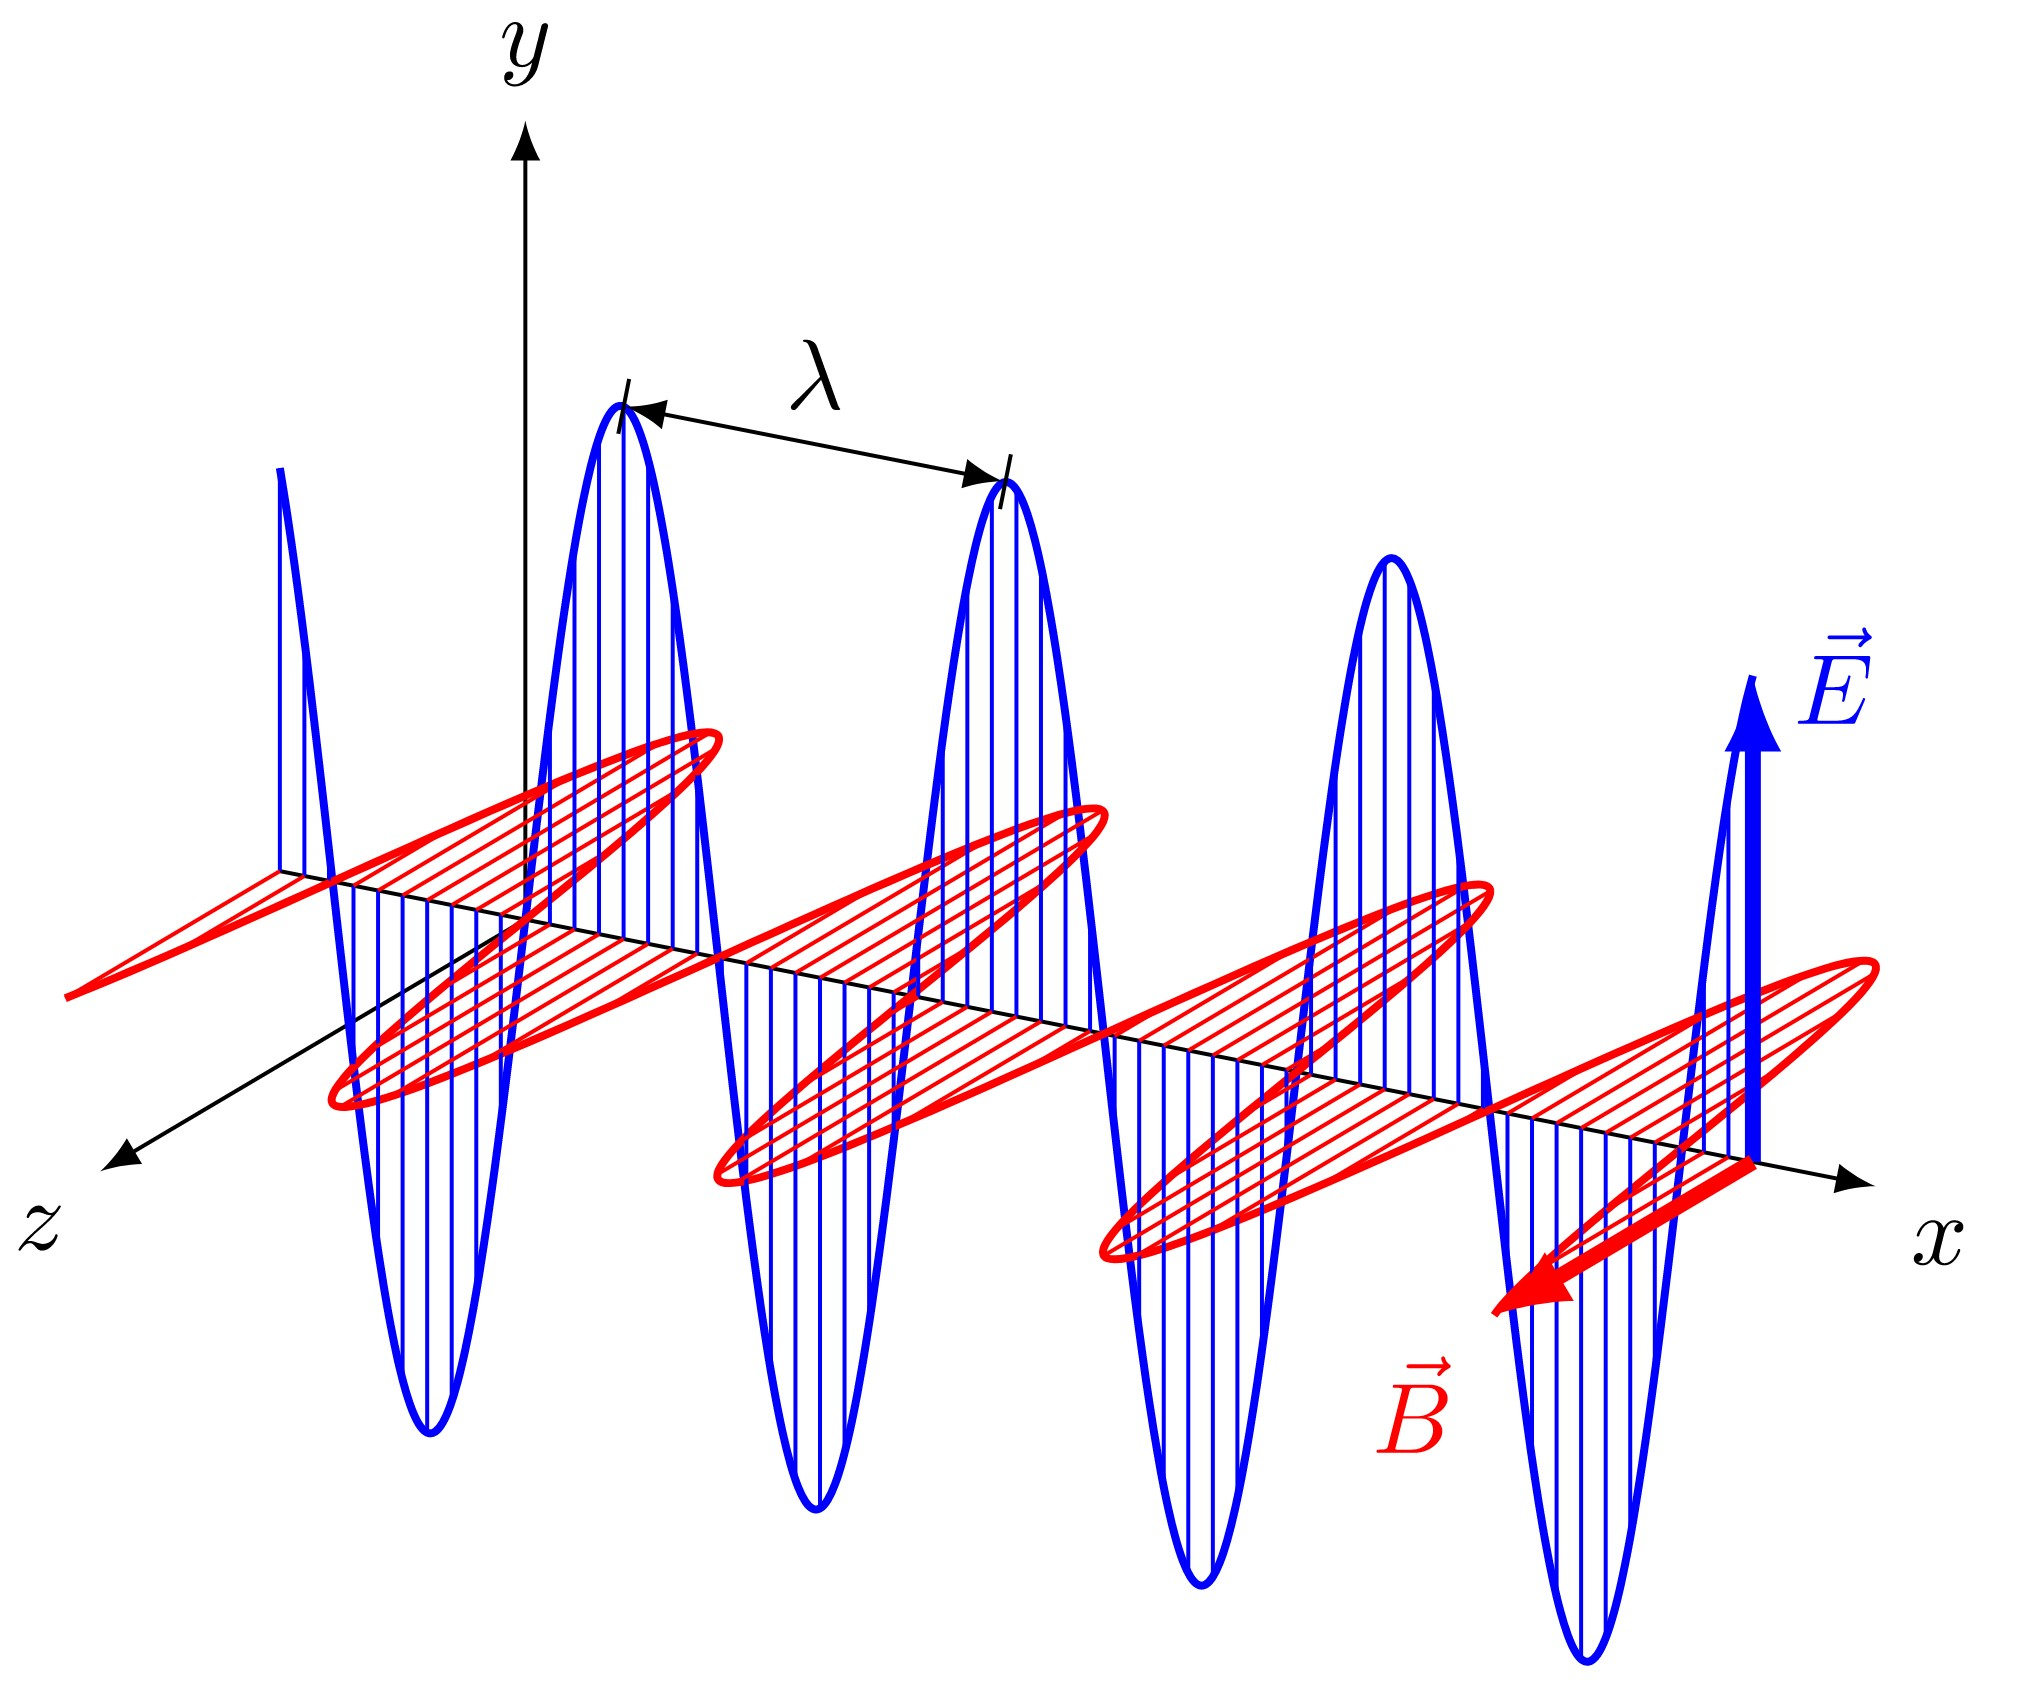
\includegraphics[width=0.8\textwidth]{elektromag.jpg}
	\caption[Ausbreitung einer elektromagnetischen Welle]{Ausbreitung einer elektromagnetischen Welle} 
	\gls{online:elektromag}
	\label{fig:elektromag}
\end{figure}
\begin{equation}
	\label{equ:lambda}
	\lambda = \frac{c}{f} 
\end{equation}
Eine solche Form von Wellen ist nicht an ein Ausbreitungsmedium gebunden, weshalb es sich auch im Vakuum (z.B. im Weltraum) ausbreiten kann. Diese Eigenschaft ermöglicht beispielsweise eine Satellitenkommunikation. Zur Erzeugung einer elektromagnetischen Welle wird zunächst eine hochfrequente Wechselspannung benötigt. Diese wird meist durch einen Quarzoszillator erzeugt. Damit sich die Welle nun ausbreiten kann, benötigt sie eine Antenne, von welcher sie sich ablösen kann.\cite{howwireless}\cite{wernerNachrichtentechnikEinfuehrungFuer2010} Um sich jedoch von einer Antenne zu lösen, muss die Wellenlänge ($\lambda$-~\ref{equ:lambda}) der elektromagnetische Welle in die Größenordnung der Antennenabmessung kommen. Da ein Ton von 300Hz jedoch nach Formel~\ref{equ:lambda} eine immens lange Antenne benötigen würde, muss mit Alternativen gearbeitet werden. Hieraus entsteht also die Bedingung, eine geeignete Trägerfrequenz zu bestimmen, um jener dann die zu versendende Information aufzumodulieren.\cite{heuermannHochfrequenztechnikKomponentenFuer2018}\cite{hoeher}
\subsection{Trägermodulation und Konstellationsdiagramm}
\label{subsec:modulationsarten}

In Kapitel~\ref{subsec:aufbauueber} wurden die Struktur und die Komponenten näher ausgeführt, welche ein Übertragungssystem besitzt. Zudem wurden elektromagnetische Wellen erklärt und die Bedeutung einer hochfrequenten Trägerfrequenz verdeutlicht. Hier soll nun die Funktionsweise eines solchen Vorhabens ausgeführt werden.  

\begin{figure}[H]
	\centering
	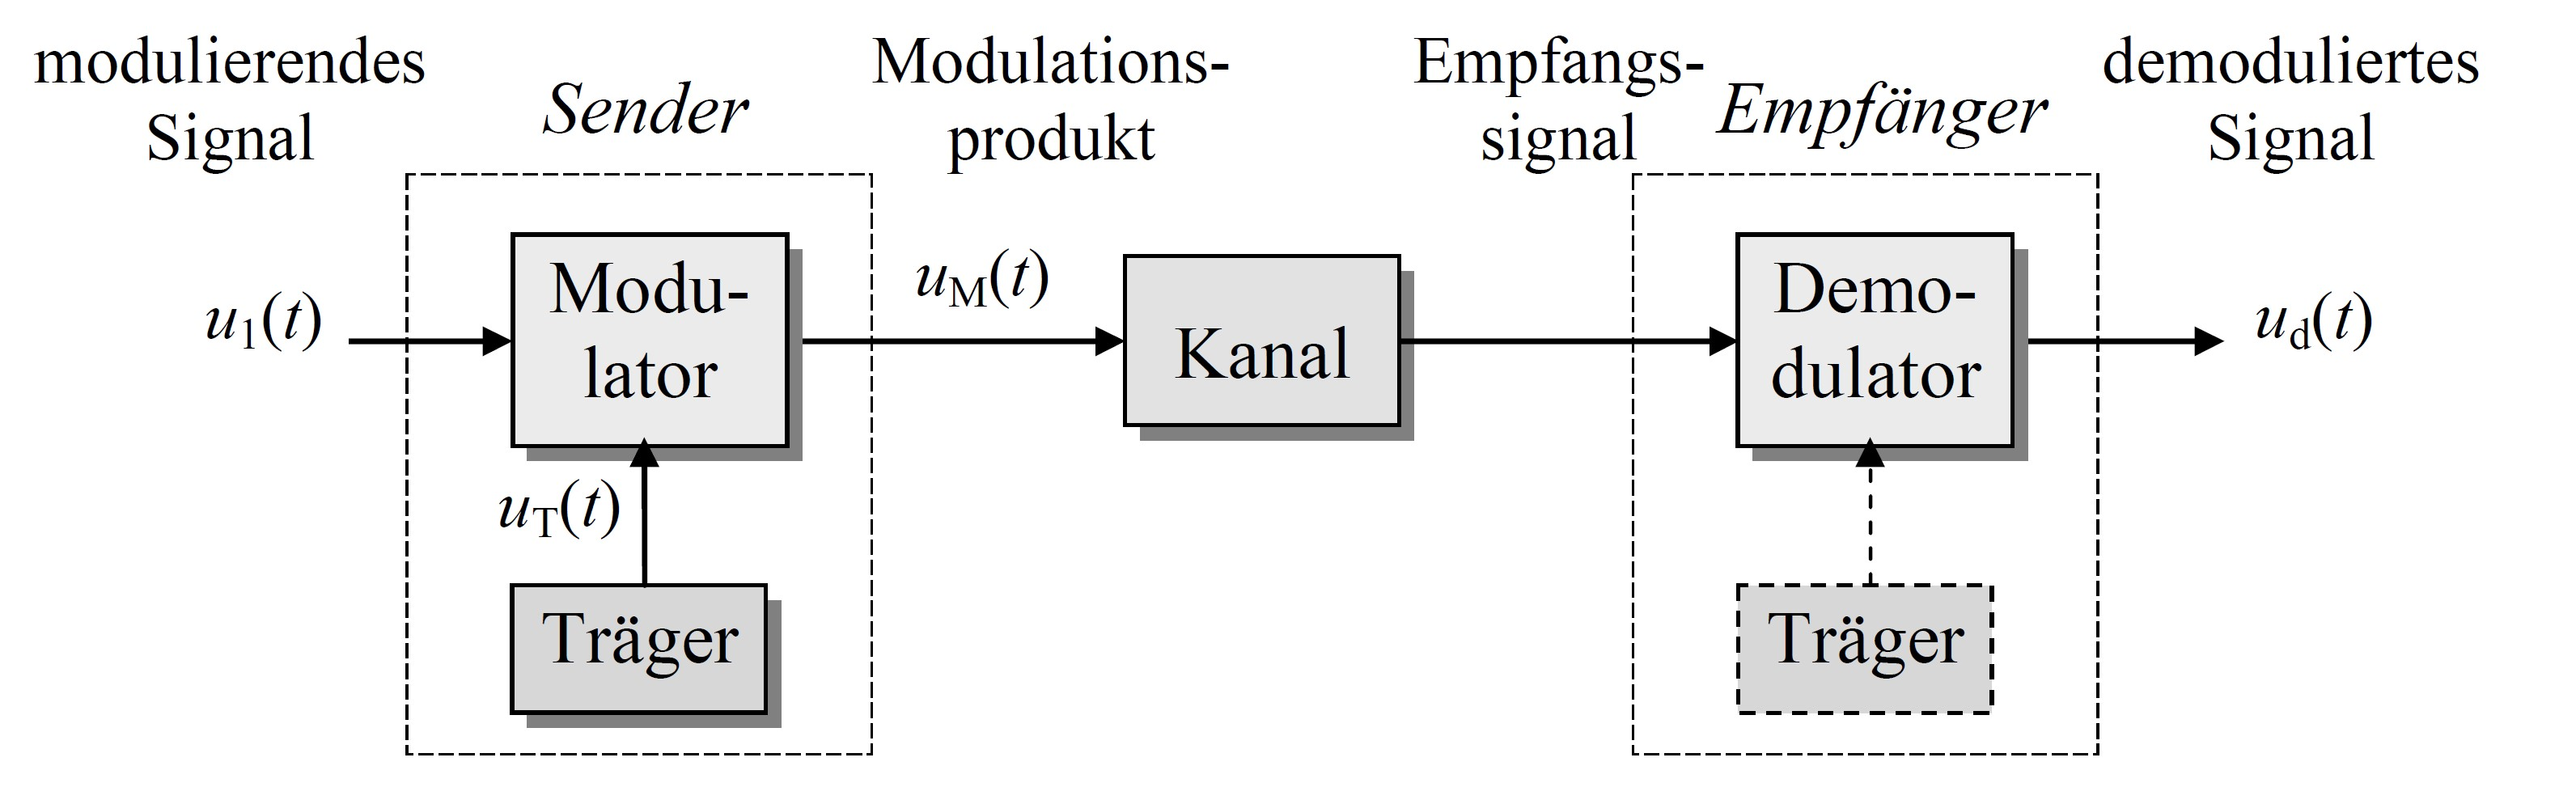
\includegraphics[width=1 \textwidth]{traegermod.jpg}
	\caption[Blockschaltbild einer Übertragung mit Trägermodulation]{Blockschaltbild einer Übertragung mit Trägermodulation} 
	\cite{wernerNachrichtentechnikEinfuehrungFuer2010}
	\label{fig:traeger}
\end{figure}
Liegt nun also ein Signal im Basisband vor, wobei es sich beispielsweise um ein Audiosignal als elektrische Spannung am Ausgang eines Mikrofons handeln könnte, wird es normalerweise in einen höheren Frequenzbereich verschoben um über eine größere Entfernung übertragen zu werden. Radio-Rundfunk liefert ein Beispiel für eine solche Trägermodulation. Hierbei macht man sich die drei variablen Parameter eines sinusförmigen Trägersignales zu eigen. Dabei handelt es sich um die Frequenz, Amplitude und Phase eines jenen. In Abhängigkeit der benutzten Verfahren spricht man von \gls{acr:AM}, \gls{acr:FM} oder \gls{acr:PM}.\cite{wernerNachrichtentechnikEinfuehrungFuer2010} Diese Theorie der Trägermodulation soll nun am Beispiel eines AM-Signals und eines FM-Signals veranschaulicht werden. 

\begin{figure}[H]
	\centering
	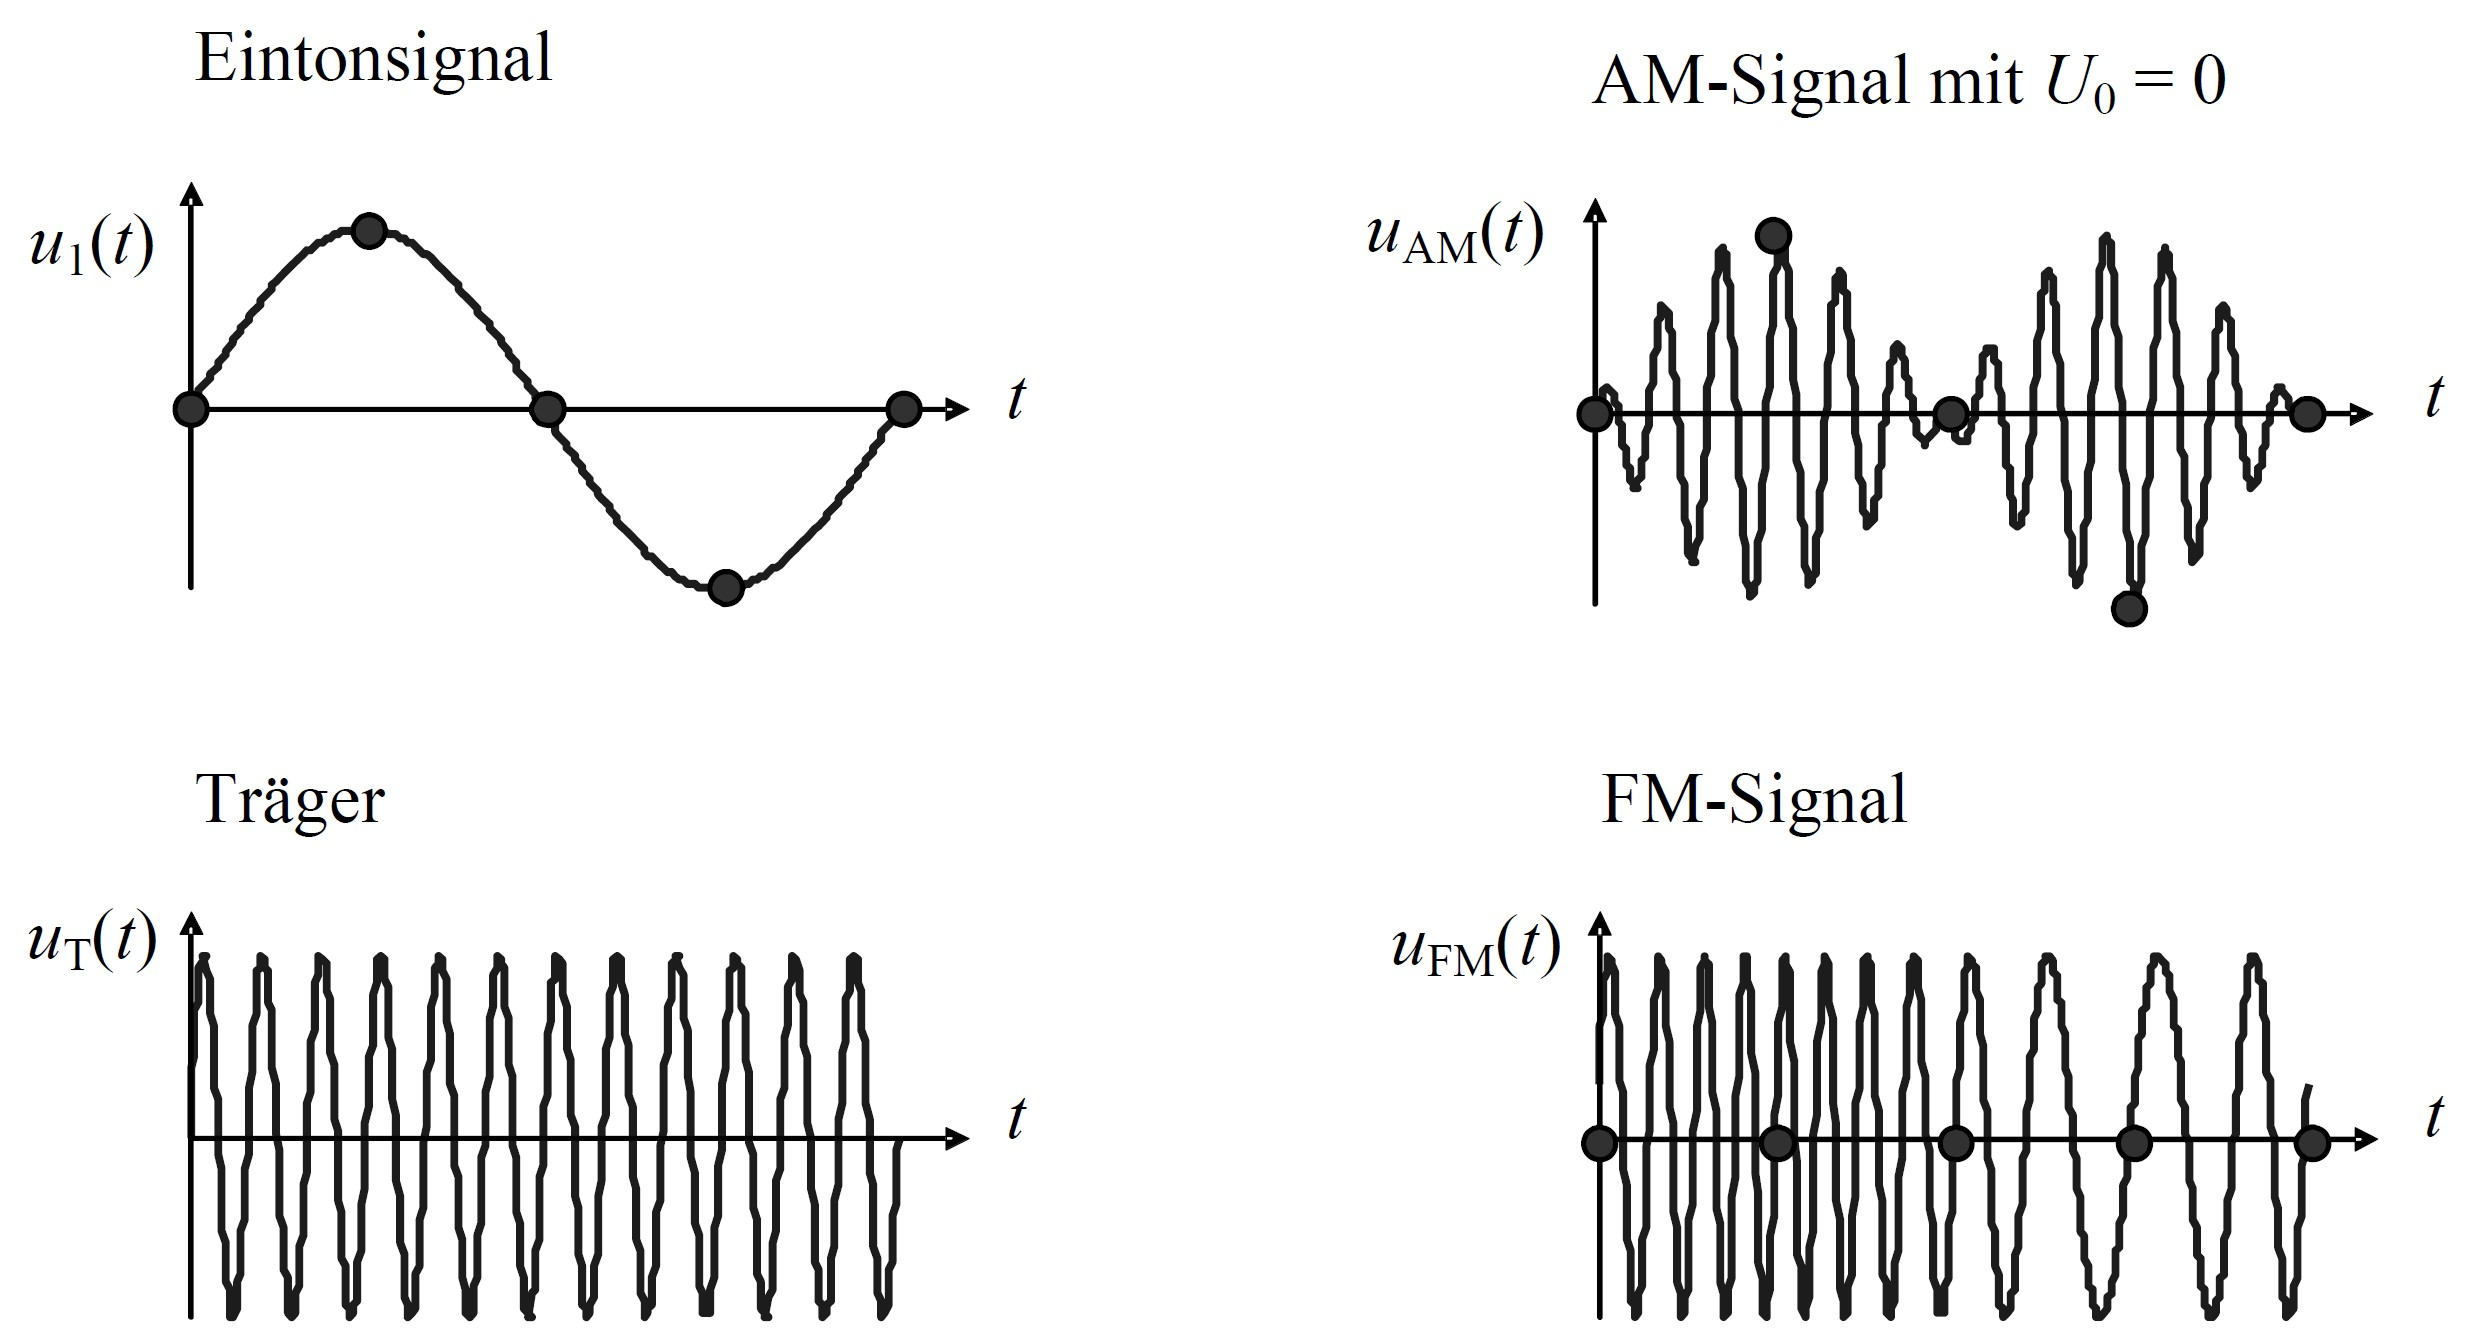
\includegraphics[width=0.85 \textwidth]{fmam.jpg}
	\caption[AM- und FM-Modulation eines Sinusträgers mit einem Eintonsignal]{AM- und FM-Modulation eines Sinusträgers mit einem Eintonsignal} 
	\cite{wernerNachrichtentechnikEinfuehrungFuer2010}
	\label{fig:fmam}
\end{figure}

Hierbei wird ein analoges Ausgangssignal verwendet. Es findet also keine Wandlung in ein digitales Signal statt. Bei der \gls{acr:AM}  die sinusförmige Trägerfrequenz mithilfe eines Mischers auf das Signal multipliziert. Dabei gibt das Eintonsignal, wie in Abbildung~\ref{fig:fmam} die Amplitude der hochfrequenten Trägerfrequenz vor und bildet somit die Einhüllende Kurve. Durch diesen Vorgang erlangt das Signal eine adäquate Frequenz zur Ablösung einer Antenne.\cite{klostermeyerDigitaleModulation2001}\cite{heuermannHochfrequenztechnikKomponentenFuer2018}

\begin{figure}[H]
	\centering
	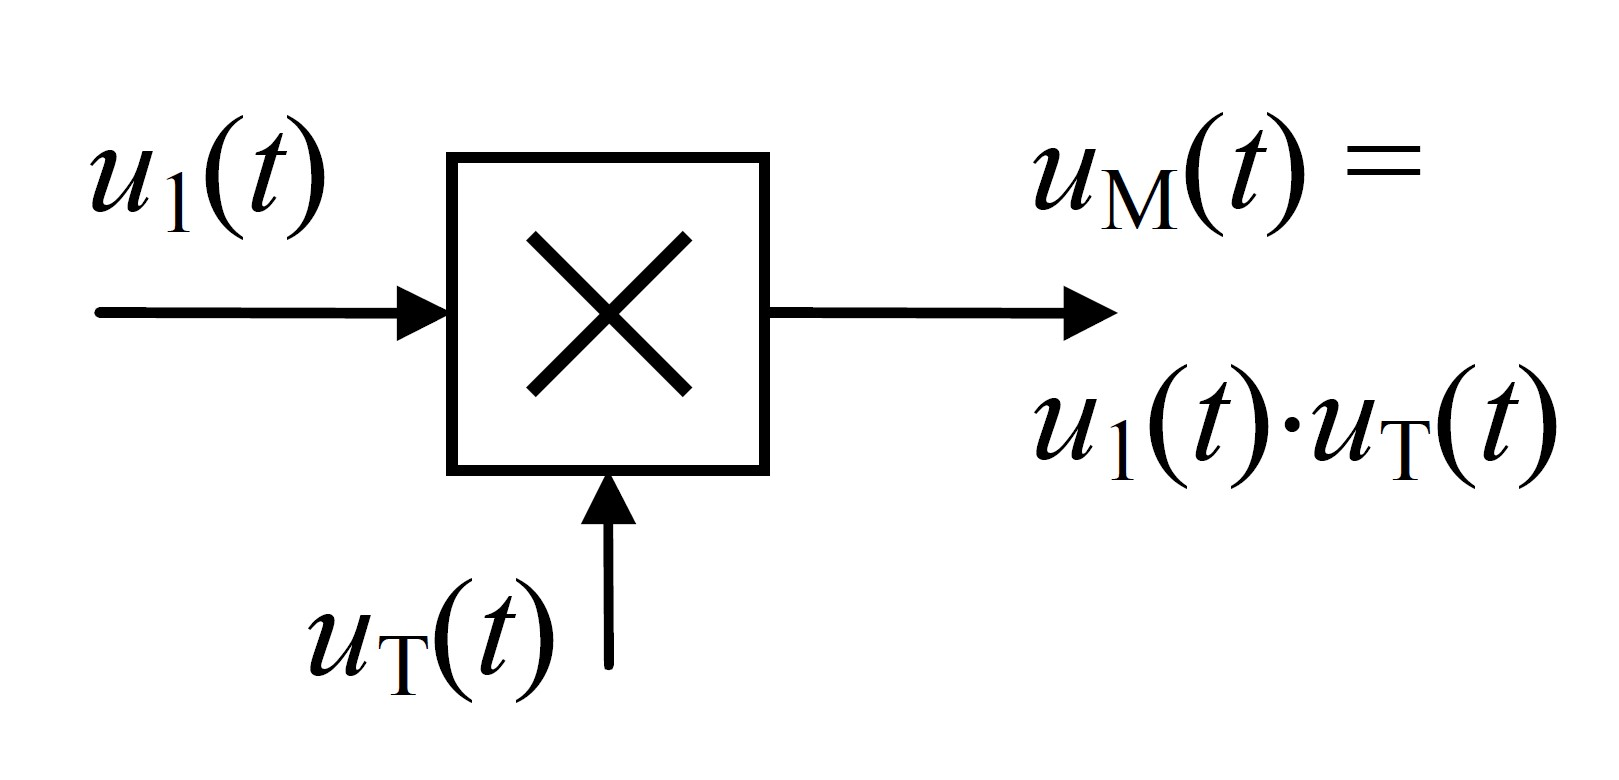
\includegraphics[width=0.3 \textwidth]{Mischer.jpg}
	\caption[Trägermultiplikation bei AM]{Trägermultiplikation bei AM} 
	\cite{wernerNachrichtentechnikEinfuehrungFuer2010}
	\label{fig:mischer}
\end{figure}

Bei Frequenzmodulation wiederum liegt die Information in der Frequenz und nicht in der Amplitude. Abbildung~\ref{fig:fmam} illustriert dies. Beim frequenzmodulierten Signal ändert sich nämlich lediglich die Trägerfrequenz, wodurch diese Art von Modulation Störungen gegenüber deutlich resistenter ist, da keine so starke Amplitudenschwankungen auftreten.\cite{hoeher}


Zur Vertiefung des Basiswissen werden nun noch digitale Modulationsarten erläutert. Hierbei wird auch mit der Variation von Frequenz, Amplitude und Phase gearbeitet. Diese drei Grundmodulationsarten sind in ihrer zweiwertigen Form in Darstellung~\ref{fig:welle} veranschaulicht.

\begin{figure}[H]
	\centering
	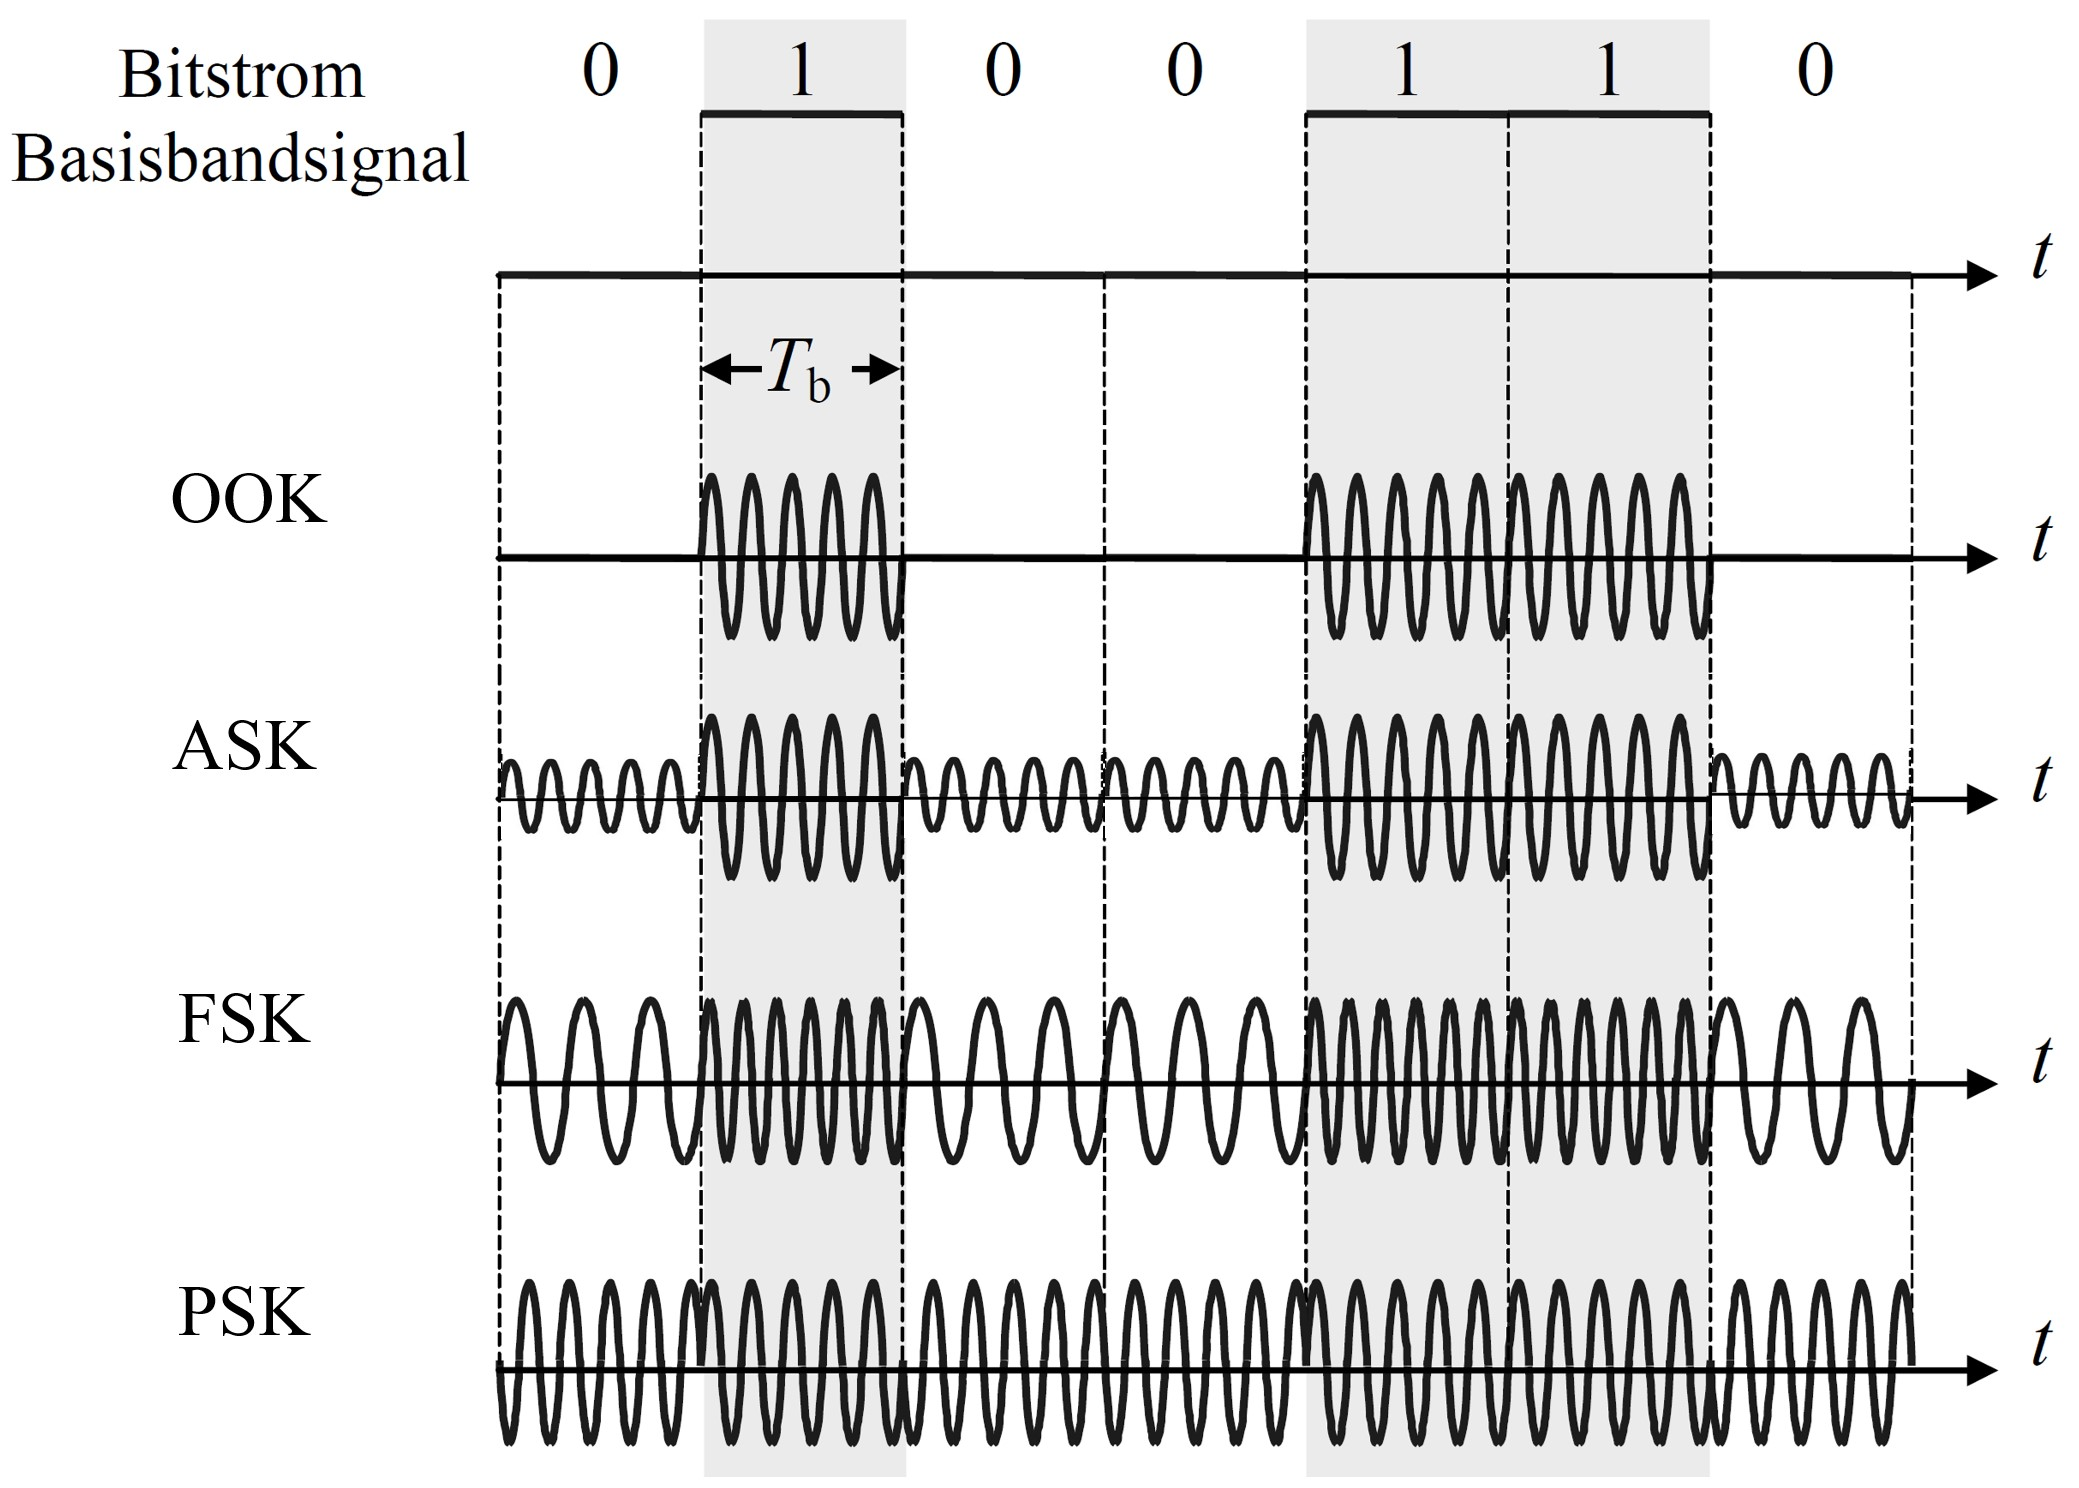
\includegraphics[width=0.9 \textwidth]{welle.jpg}
	\caption[Binäre Übertragung mit Sinusträger]{Binäre Übertragung mit Sinusträger} 
	\cite{wernerNachrichtentechnikEinfuehrungFuer2010}\gls{online:Eigen}
	\label{fig:welle}
\end{figure}

Hierbei wurde noch eine weitere Version der \gls{acr:AM}-Modulation illustriert. Diese nennt sich \gls{acr:OOK} und hat bei der Übertragung einer 1 eine Amplitude und wird jedoch bei der Übertragung einer 0 auf Null gesetzt. Da unter diesen Voraussetzungen nicht ermittelt werden kann wann die Übertragung endet, wird hier ein Zwischenwert mit z.B. halber Amplitude zum Senden einer 0 verwendet.
Die übertragenen Bit werden hierbei auch Symbole genannt. Modernere Kommunikationssysteme verwenden mittlerweile jedoch Modulationsarten die es ermöglichen mehrere Bits pro Symbol zu übertragen. Bei zwei Bit werden hierbei vier Zustände benötigt. Daraus entstehen dann Erweiterungen der genannten Modulationsarten, welche 4-\gls{acr:ASK} 4-\gls{acr:FSK} und 4-\gls{acr:PSK} bezeichnet werden. Oft wird die Ziffer Vier auch mit dem Buchstaben Q fur Quadratur ersetzt.\cite{howwireless}\cite{butlerWirelessNetworkingDeveloping2013} Bei einer \gls{acr:QAM} wird beispielsweise eine Kombination zweier Modulationsarten verwendet. Dabei werden sowohl die Amplituden- als auch Phasenmanipulation benutzt, um Informationen zu modulieren. 

Da im Zuge dieser Abschlussarbeit größtenteils mit einer \gls{acr:QAM}-Modulaton gearbeitet wurde, wird diese näher erläutert. Um jedoch ein besseres Verständnis für den Aufbau einer solchen Modulation zu erlangen, muss der Begriff des Konstellationsdiagramms eingeführt werden. Dies soll am Beispiel einer \gls{acr:QPSK} veranschaulicht werden. Modulierte Wellen, sind sinusförmig und wie folgt definiert. 

\begin{equation}
	\label{equ:qpsk}
	s_{i}(t) = A \cdot cos(\omega \cdot t+\varphi_{0}+\varphi_{i})
\end{equation}

Dabei steht die Variable $A$ für eine, bei der \gls{acr:QPSK}, konstante Amplitude. Die variable $\varPhi_{0}$ beschriebt zusätzlich die Phase des Referenzsignals.Zudem ergibt sich die in Formel ~\ref{equ:qpsk} genannte Kreisfrequenz $\omega$ aus:

\begin{equation}
	\label{equ:qpsk}
	\omega = 2 \cdot \pi \cdot f
\end{equation}
Um die Entfernung der Symbole zu maximieren werden diese bei der \gls{acr:QPSK} um 90$^\circ$ zueinander verschoben. Tabelle~\ref{tab:qpsk} gibt Information über die verschiedenen Phasenlagen die von $i$ angenommen werden können.
\begin{table}[htb]
	\begin{center}
		\begin{tabular}[h]{cc}	
			\toprule
			Funktion & Phase  \\
			\midrule
			$s_{1}(t)$ & $0^\circ$ \\
			$s_{2}(t)$ & $90^\circ$ \\
			$s_{3}(t)$ & $180^\circ$ \\
			$s_{4}(t)$ & $270^\circ$ \\
			\bottomrule
		\end{tabular}
		\caption{Phasenlagen bei der \gls{acr:QPSK}
		\label{tab:qpsk}
	\end{center}
\end{table}

\subsection{OFDM}
\label{subsec:Unterabschnitt1}



\subsection{DRM}
\label{subsec:Unterabschnitt1}



\section{Elektrische Bauteile}
\label{subsec:Unterabschnitt1}
In diesem Kapitel werden grundlegende Bauteile eines \gls{acr:VLC}-Senders dargestellt und näher erläutert. Diese sind essenziell, um die Datenübertragung mittels dem optischen Kanal zu ermöglichen.

\subsection{Leuchtdiode}
\label{sub:led}

Eine \gls{acr:LED} ist ein Licht-emittierendes Halbleiter-Bauelement mit einem pn-Übergang. Ihre elektrischen Eigenschaften stimmen mit der einer Standard Diode überein, wodurch sie in nur eine Richtung leitend ist und in die entgegengesetzte Stromrichtung sperrt. Wenn durch einen eingekoppelten elektrischen Strom die \gls{acr:LED} in Durchlassrichtung betrieben wird, findet eine Lichtemission statt.\cite{slabke} 

\begin{figure}[H]
	\centering
	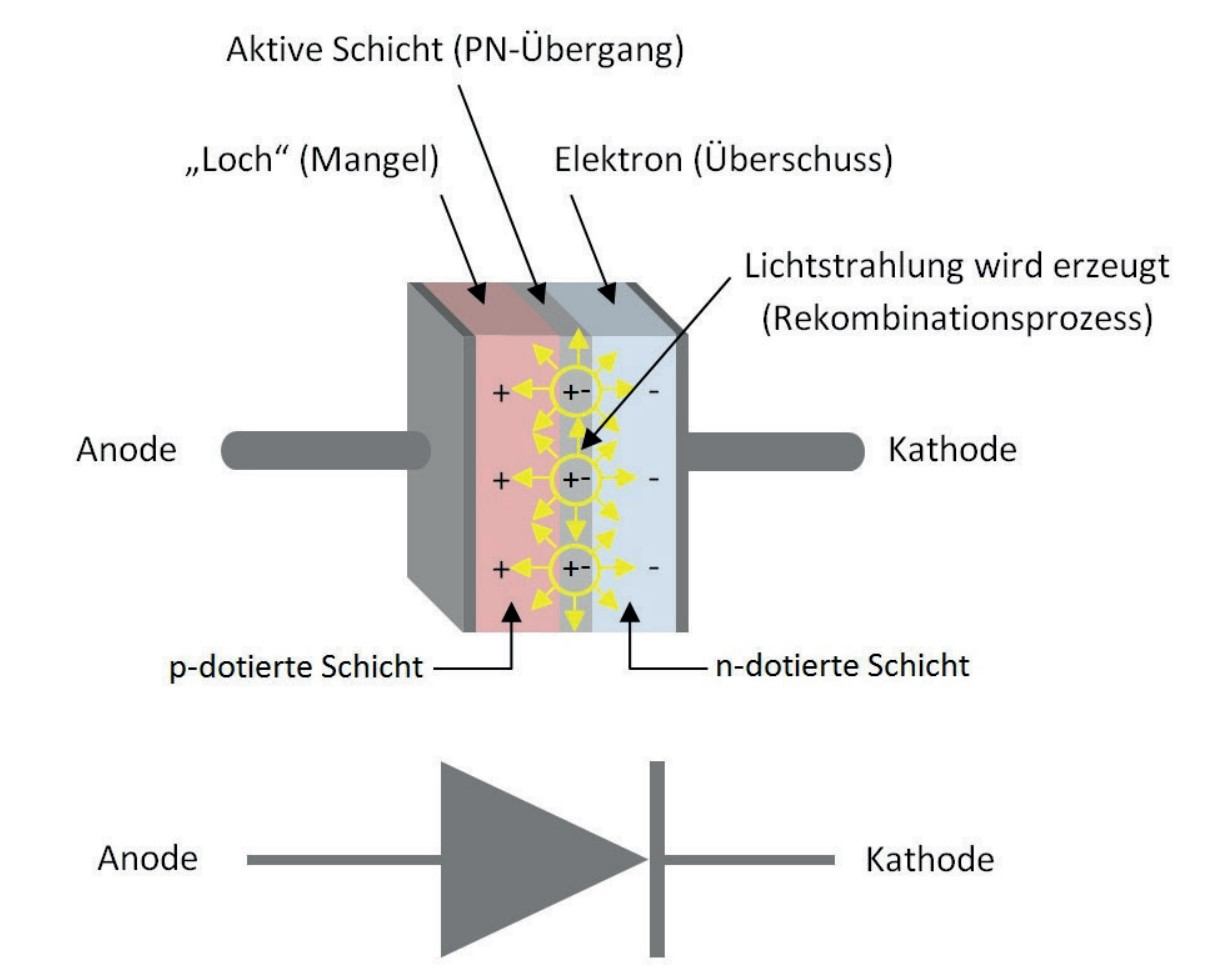
\includegraphics[width=0.65 \textwidth]{LED.jpg}
	\caption[Strahlungserzeugung in der LED am pn-Übergang]{Strahlungserzeugung in der LED am pn-Übergang} \cite{slabke}
	\label{fig:LED}
\end{figure}

Der Grundsatz der Lichterzeugung in einer \gls{acr:LED} beruht auf einem Halbleiterkristall, der durch das Einbringen von Fremdatomen so dotiert ist, dass in der Diode zwei Gebiete entstehen. In einem Gebiet entsteht ein Elektronenüberschuss und in dem anderen Gebiet entstehen Löcher. Durch das Injizieren von Elektronen aus der positiv dotierten Seite in die Sperrschicht rekombinieren sich Löcher und Elektronen, wodurch Energie in Form von Licht abgegeben wird.\cite{slabke} Die Farbe hängt dabei vom Halbleitermaterial und der genauen Dotierung ab. Zudem ist dieser Rekombinationsprozess stark temperaturabhängig. Dies wird in einem noch folgenden Kapitel näher erläutert.

\begin{figure}[H]
	\centering
	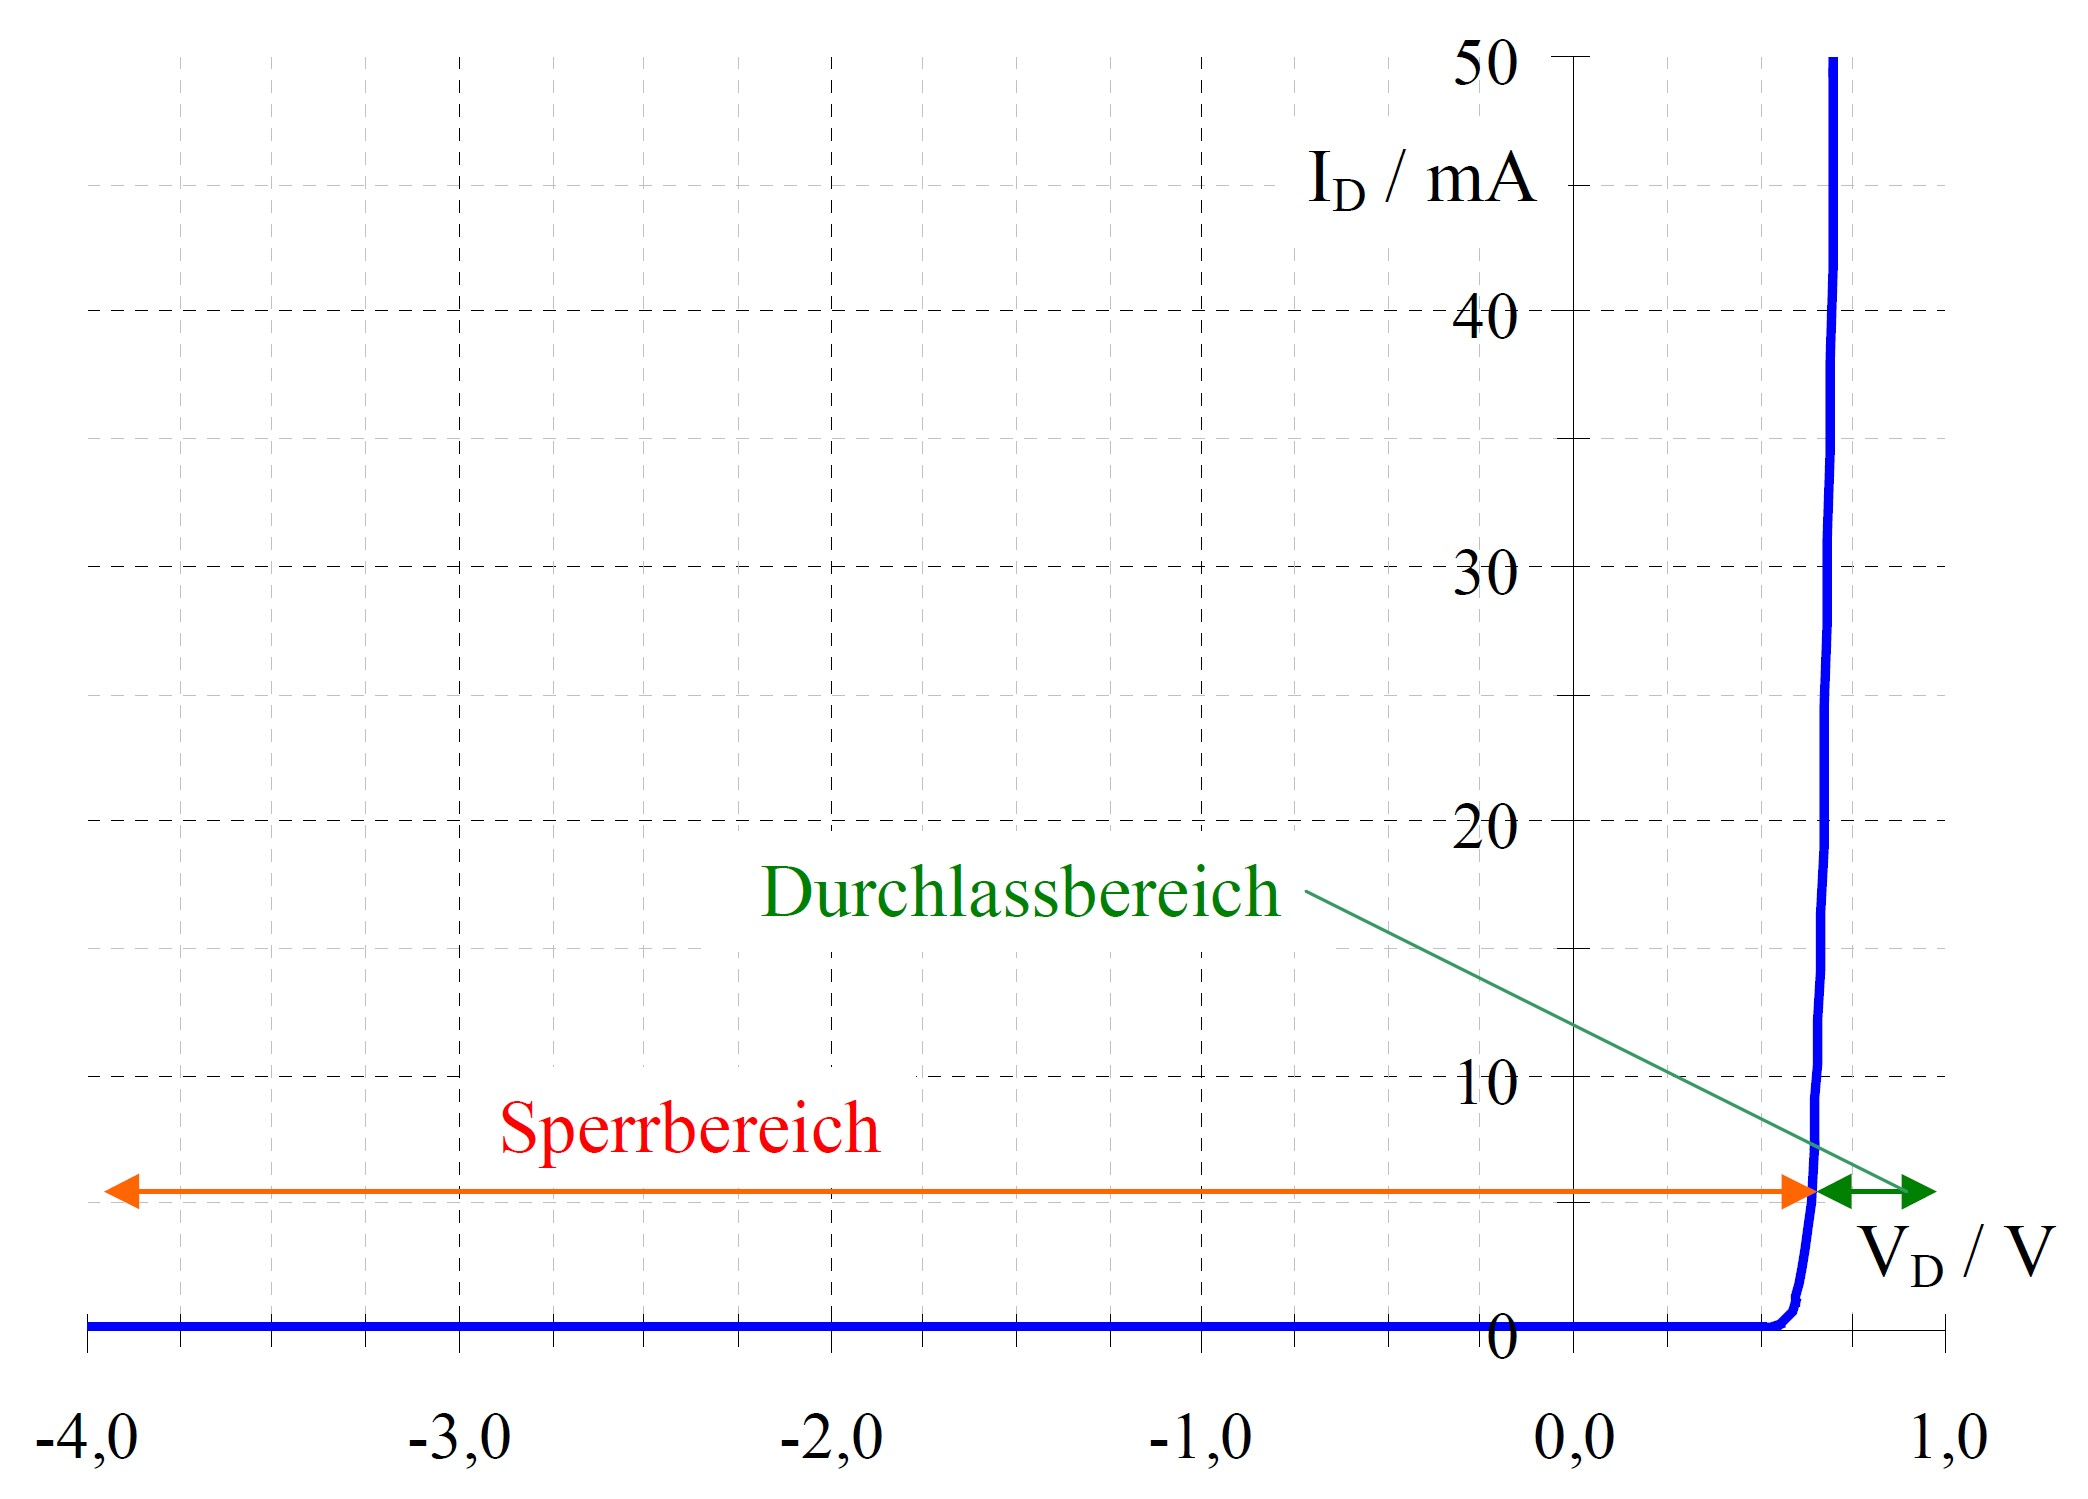
\includegraphics[width=0.65 \textwidth]{Kennlinie.jpg}
	\caption[Diodenkennlinie]{Diodenkennlinie} 
	\gls{online:elektronik}
	\label{fig:Kennlinie}
\end{figure}


In der Abbildung ~\ref{fig:Kennlinie} ist die Strom-/Spannungskennlinie einer Diode in Durchlassrichtung
dargestellt. Die Kennlinie einer LED hat den selben Verlauf, jedoch ist die Durchlassspannung
je nach gewählter Farbe nicht bei ca. 0.7V sondern bei bis zu 4V bei
einer blauen LED. 

\begin{figure}[H]
	\centering
	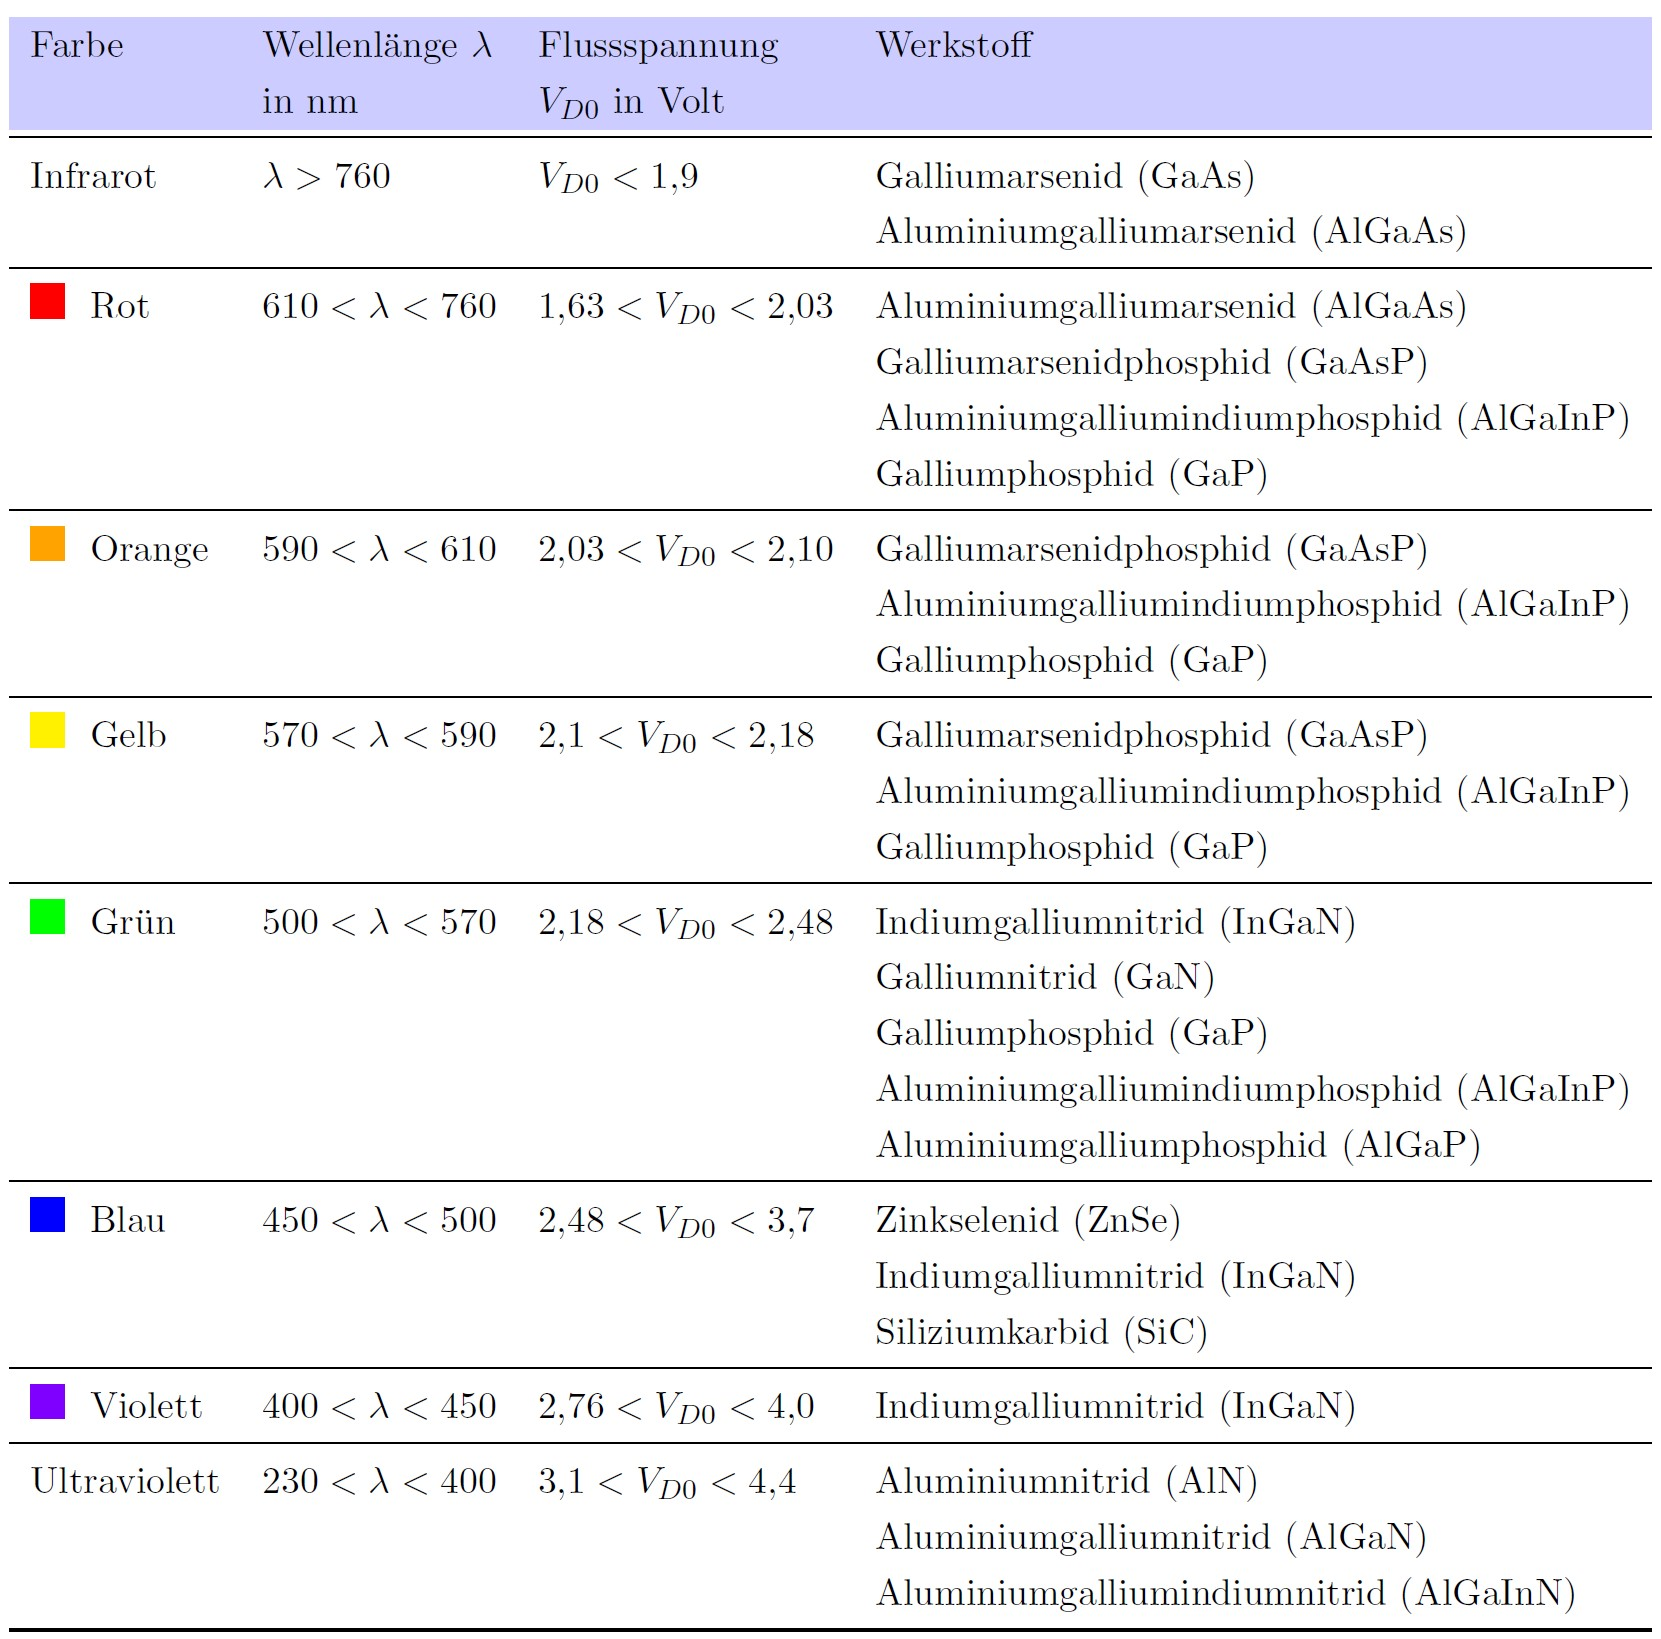
\includegraphics[width=0.85 \textwidth]{Flussspannung.jpg}
	\caption[Flussspannungen von \gls{acr:LED}s verschiedener Farben]{Flussspannungen von \gls{acr:LED}s verschiedener Farben} 
	\gls{online:elektronik}
	\label{fig:Flussspannung}
\end{figure}

Wie in Abbildung ~\ref{fig:Kennlinie} illustriert ist, ändert sich die Spannung in ihrem Verlauf
ab einem gewissen Punkt nur noch minimal. Das bedeutet, dass sich ab einer gewissen
angelegten Spannung lediglich der Strom noch weiter erhöhen kann. Da die
Leuchtintensität der \gls{acr:LED} von dieser Höhe des Stromdurchflusses abhängt, führt dies zu der
Betrachtung, den durchfließenden Strom statt der angelegten Spannung zu regulieren.
Stellt man nun den durch die \gls{acr:LED} fließenden Strom mit der Ausgangsleistung
ins Verhältnis, ergibt sich ein Zusammenhang wie ihn Abbildung ~\ref{fig:Helligkeit} zeigt. 

\begin{figure}[H]
	\centering
	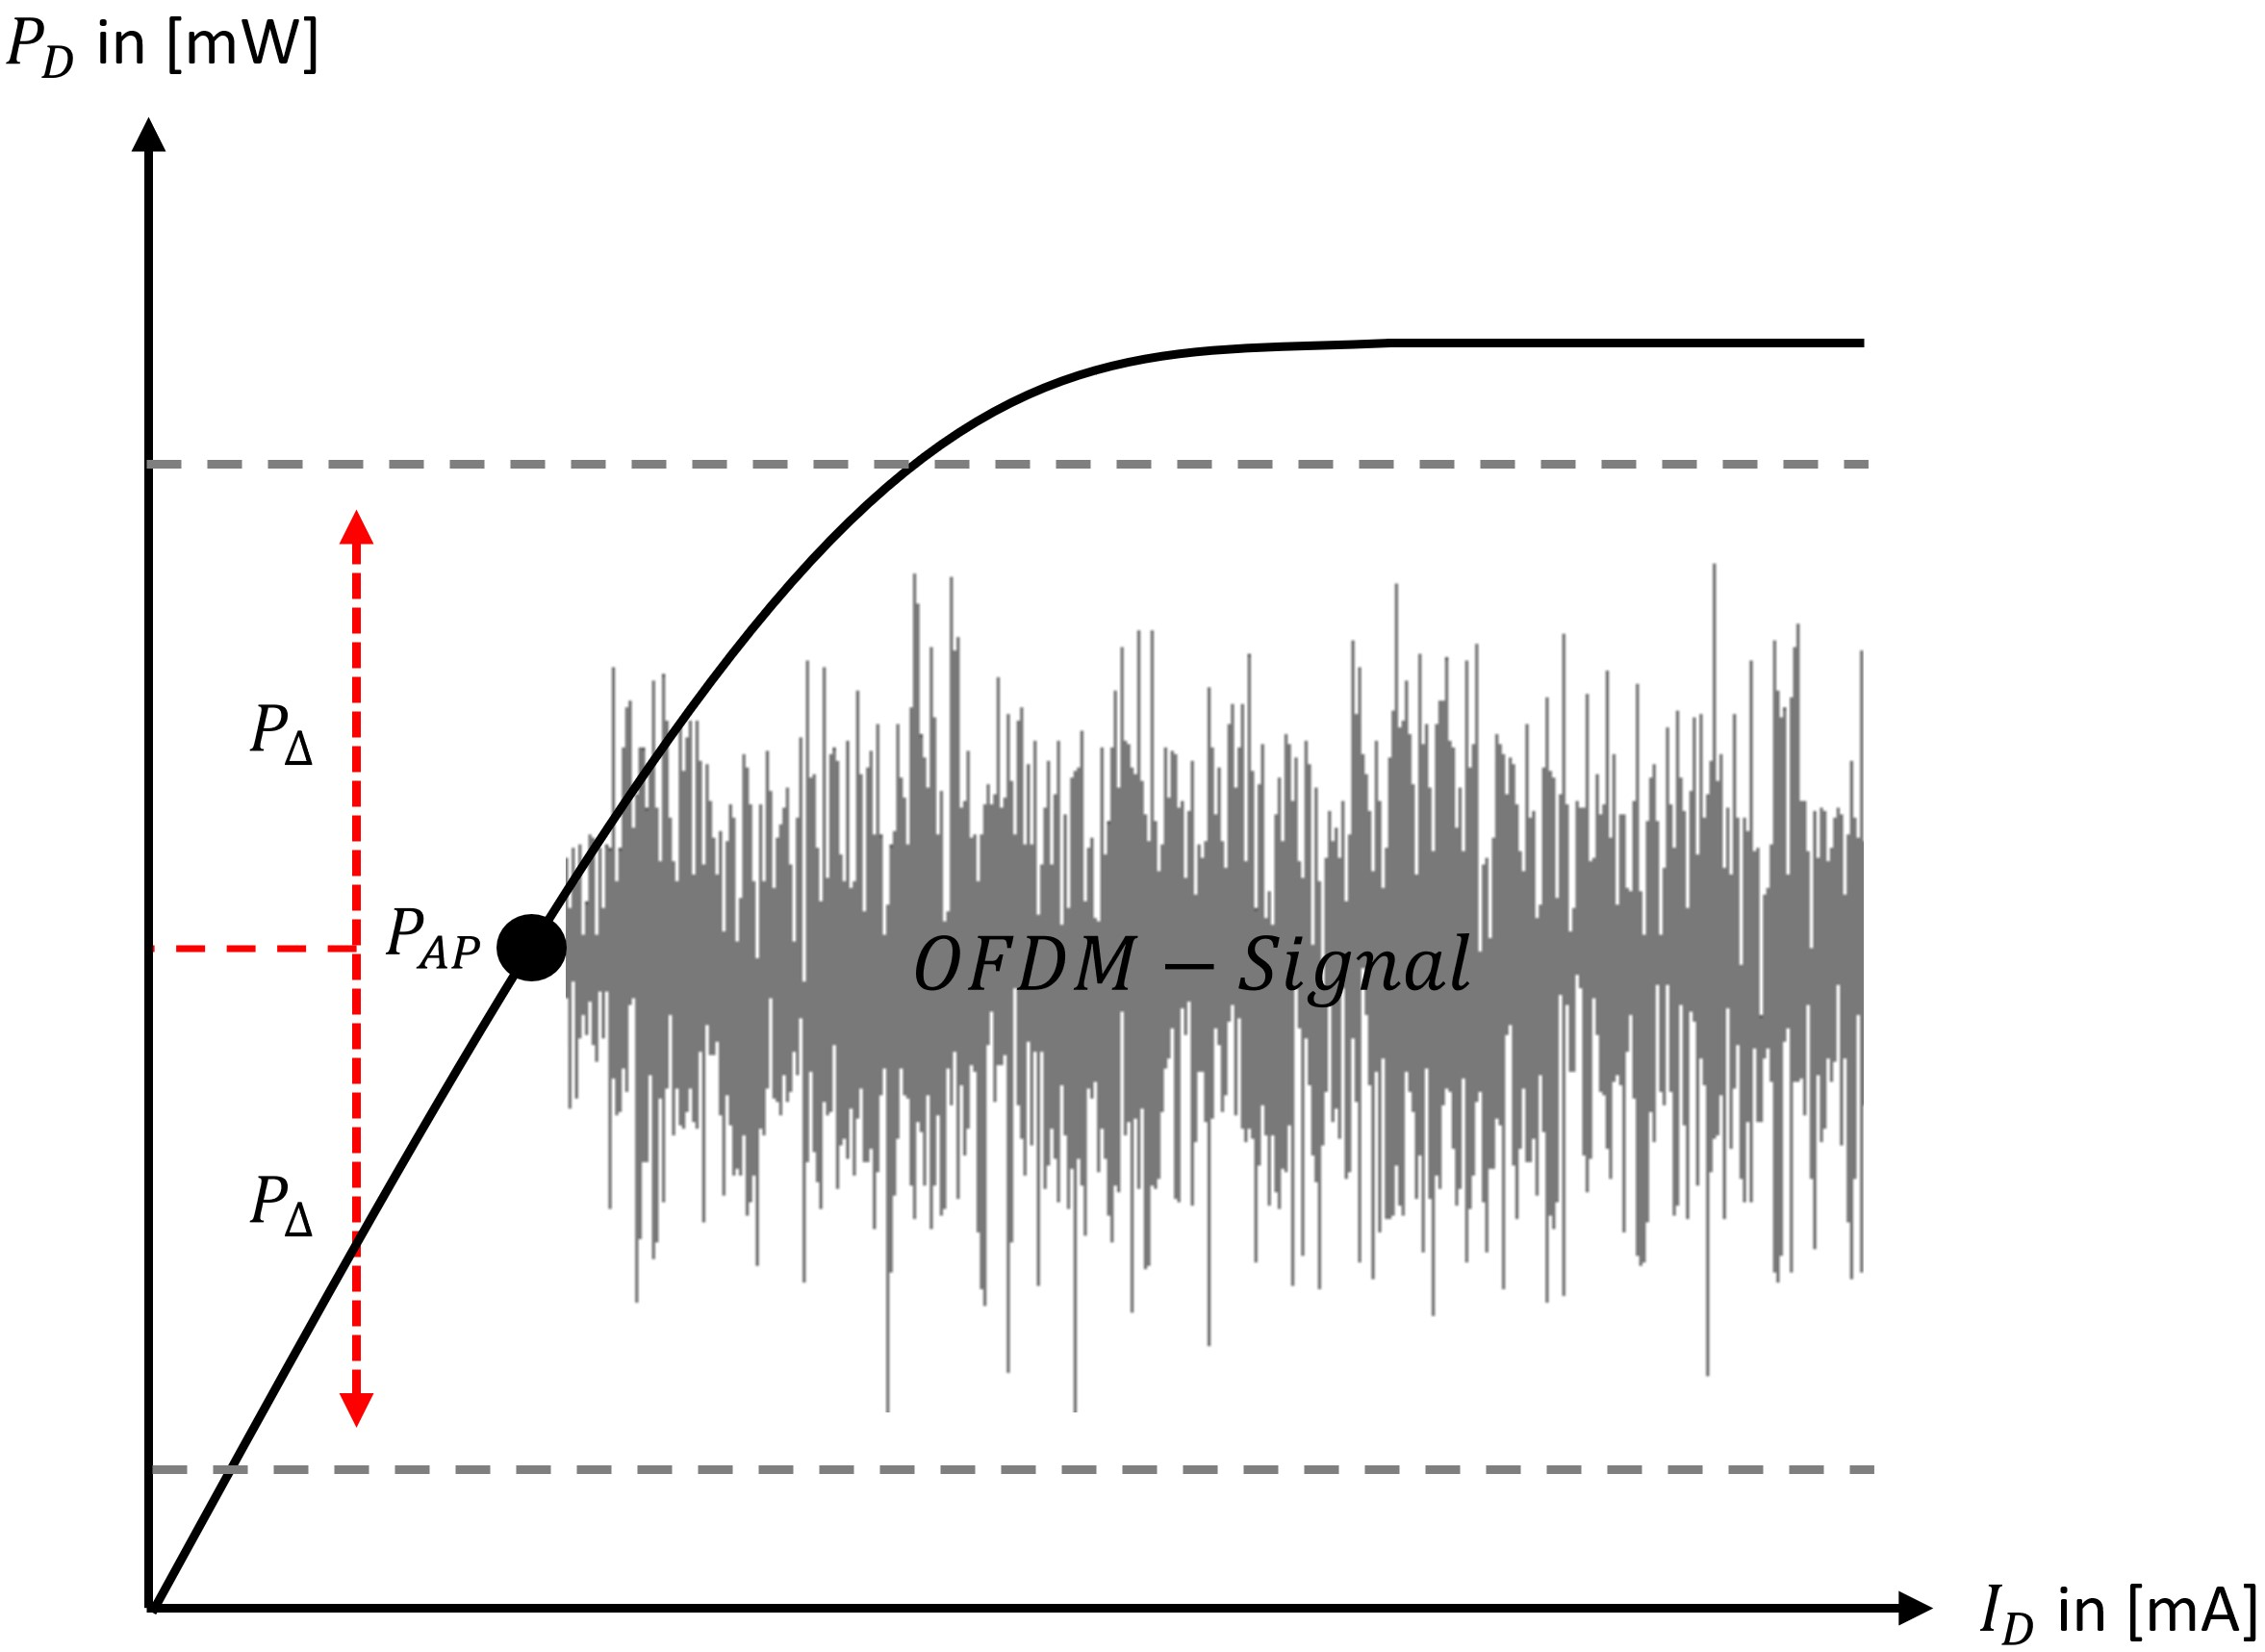
\includegraphics[width=0.78 \textwidth]{Helligkeit.jpg}
	\caption[Kennlinie einer Diode – Lichtleistung zu fließendem Strom]{Kennlinie einer Diode – Lichtleistung zu fließendem Strom} 
	\gls{online:Eigen}
	\label{fig:Helligkeit}
\end{figure}

An dieser Stelle wird verdeutlicht, dass es zwei außerordentlich nicht-lineare Abschnitte in der Kennlinie gibt, welche sich durch ihre stark nicht-linearen Eigenschaften keineswegs zur Datenübertragung eignen. Zwischen diesen Bereichen, um die etwa mittlere Lichtleistung, gibt es jedoch einen linearen Bereich, welcher sich ausgezeichnet für die Übertragung von Daten eignet. Dies bedeutet, dass die LED auf einem festen Arbeitspunkt AP betrieben werden muss. Dieser Arbeitspunkt liefert der Diode einen immensen Aktionsradius, wodurch eine maximale Aussteuerung der Amplitude des Signals und somit eine verbesserte Konstellation zur Signalübertragung gewährleistet wird.


\subsection{Operationsverstärker}
\label{subsec:OP}

„Im Grunde besteht kein Unterschied zwischen einem normalen Verstärker und einem Operationsverstärker. Beide dienen dazu, Spannungen bzw. Ströme zu verstärken. Während die Eigenschaften eines normalen Verstärkers jedoch durch seinen inneren Aufbau vorgegeben sind, ist ein Operationsverstärker so beschaffen, dass seine Wirkungsweise überwiegend durch eine äußere Gegenkopplungs-Beschaltung bestimmt werden kann. Um dies zu ermöglichen, werden Operationsverstärker als gleichspannungsgekoppelte Verstärker mit hoher Verstärkung ausgeführt. Damit keine zusätzlichen Maßnahmen zur Arbeitspunkteinstellung erforderlich werden, verlangt man ein Eingangs- und Ausgangsruhepotential von 0V. Deshalb sind in der Regel zwei Betriebsspannungsquellen erforderlich: eine positive und eine negative.“(\cite{tietzeElectronicCircuits2008},S.491)

Ein \gls{acr:OP} kann also mit einem Differenzverstärker von theoretisch unendlicher Verstärkung verglichen werden. Diese bezeichnet man als Leerlaufverstärkung. Schließlich führt das dazu, dass eine Gesamtverstärkung der Schaltung von einer zusätzlichen externen Verdrahtung abhängt. Diese wird von einem rückgekoppelten Netzwerk hergestellt und nennt sich Schleifenverstärkung.\cite{lutzHalbleiterLeistungsbauelemente2012}

\begin{figure}[H]
	\centering
	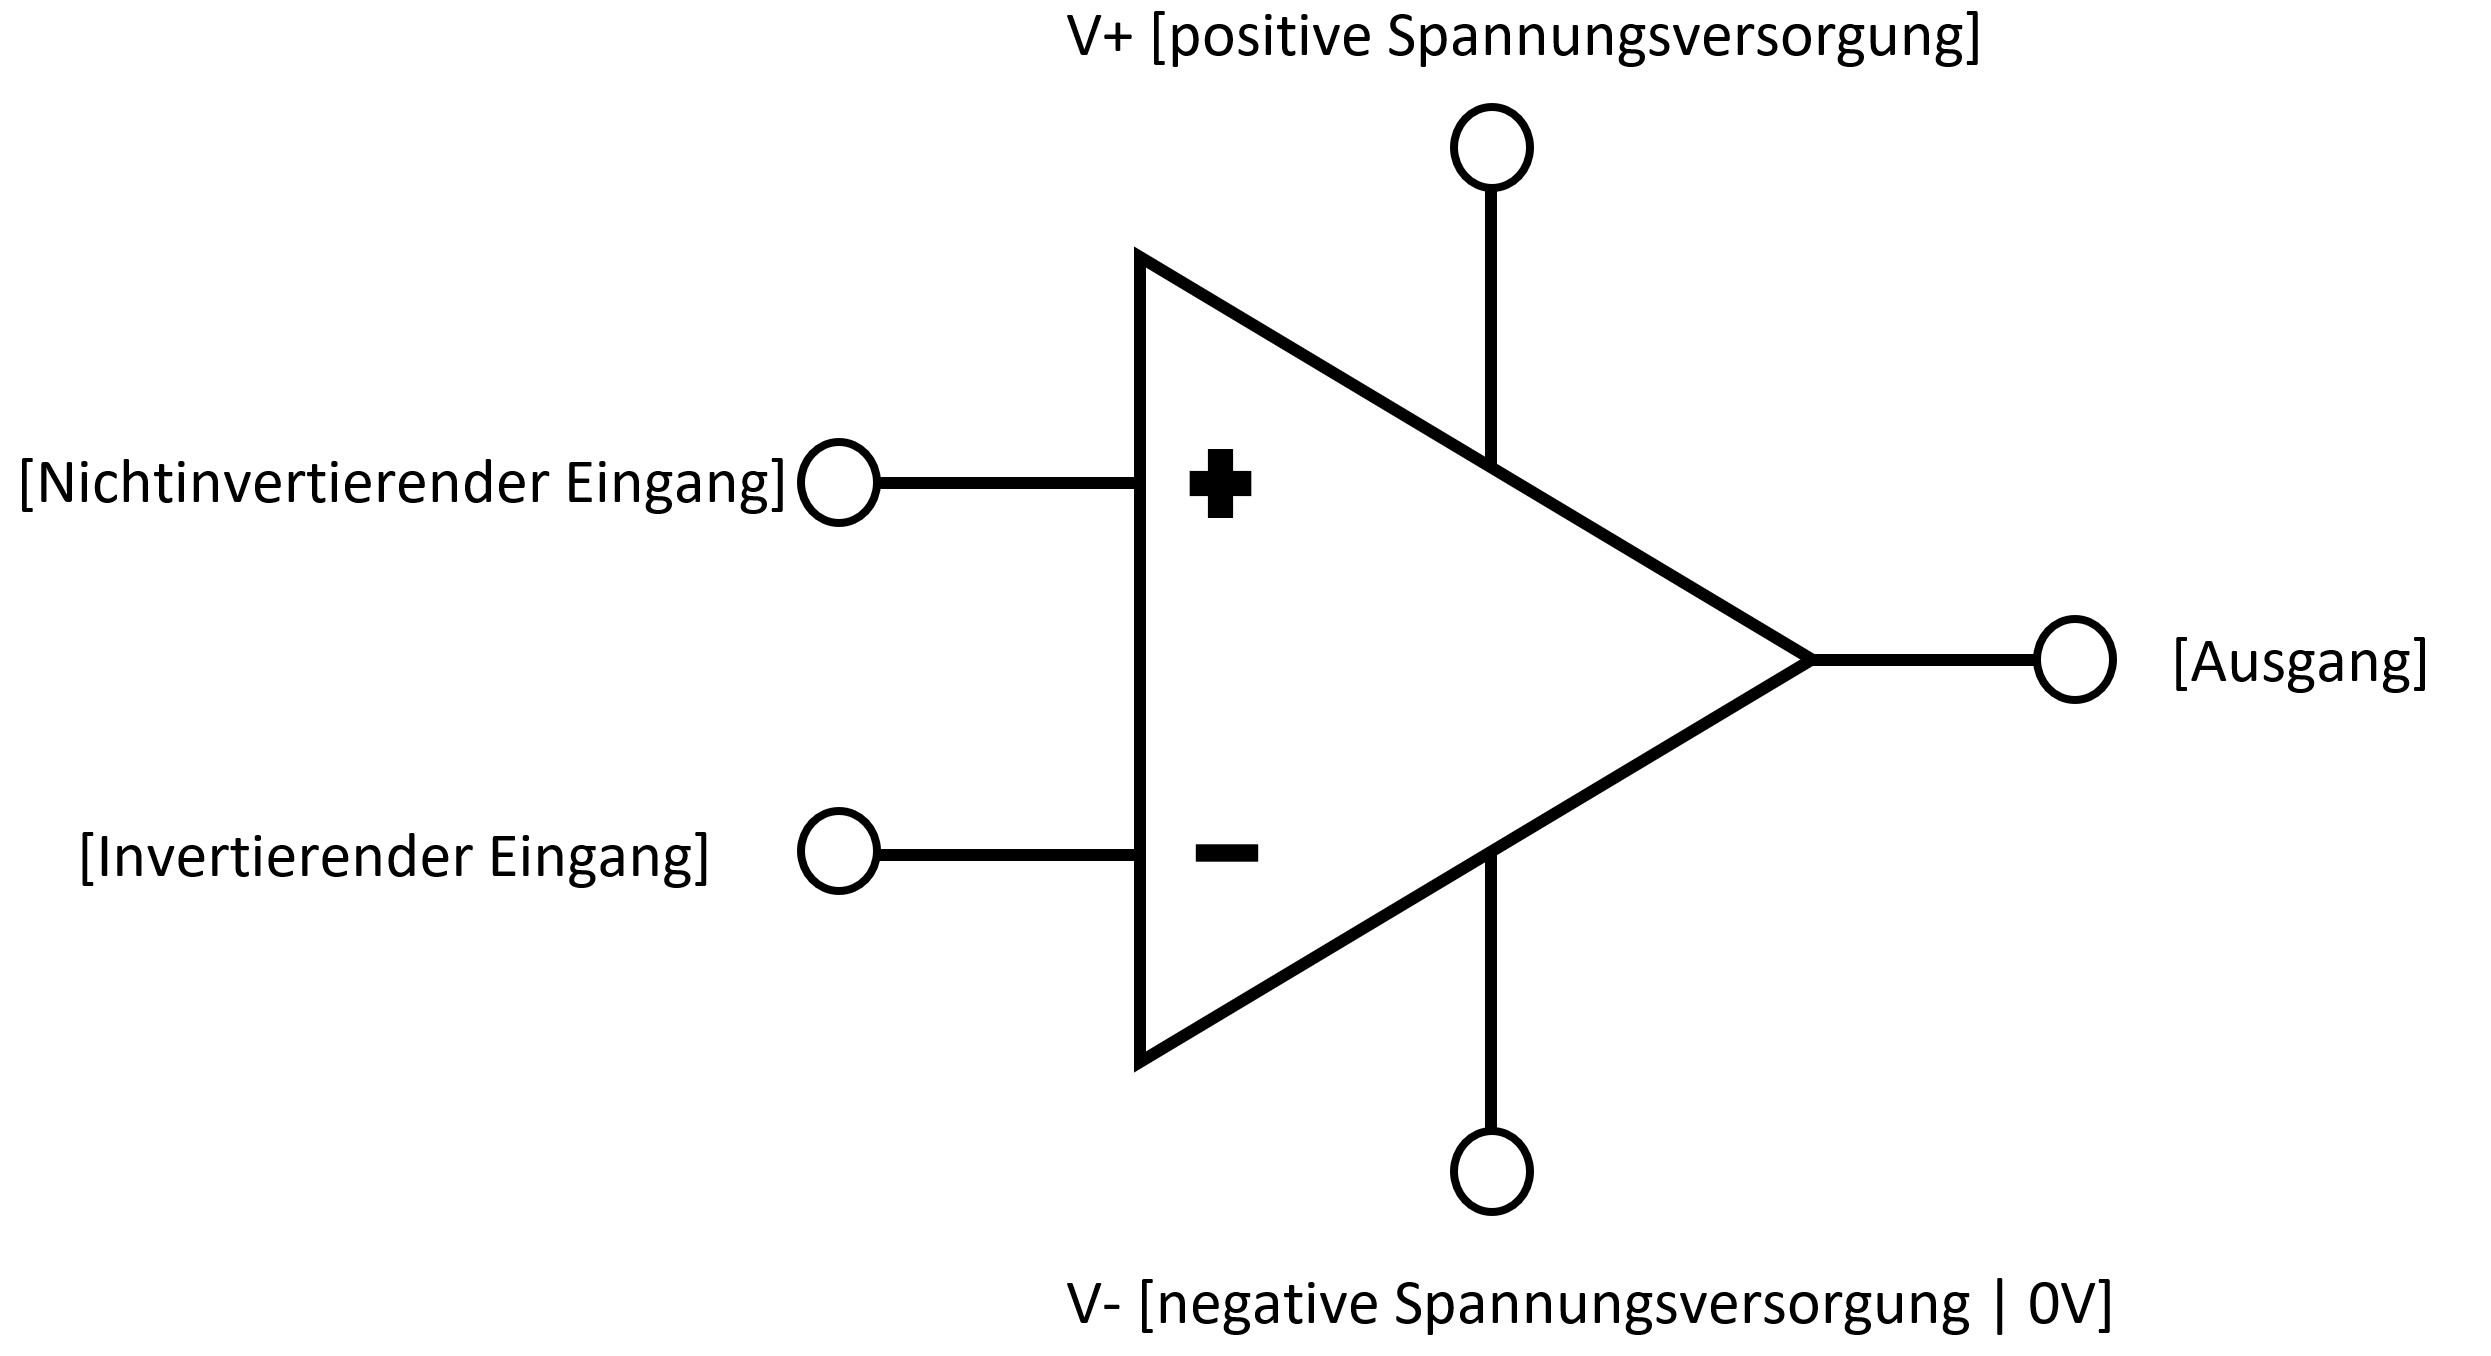
\includegraphics[width=0.7 \textwidth]{OPV.jpg}
	\caption[Operationsverstärker Anschlussschema]{Operationsverstärker Anschlussschema} 
	\gls{online:Eigen}
	\label{fig:OPV}
\end{figure}

Sie werden im Allgemeinen in Form einer integrierten Schaltung (\gls{acr:IC}) hergestellt, da die in dem Datenblatt eines Operationsverstärkers angegebenen Werte ausreichend beschrieben werden. Zudem verfügt der \gls{acr:OP} über einen invertierenden (-) und nicht-invertierenden (+) Eingang. Daraus können zwei der \gls{acr:OP}-Grundschaltungen extrahiert werden. Um das Verhältnis zwischen der Ausgangsspannung $U_{a}$ und der Eingangsspannung $U_{e}$ zu berechnen werden häufig die Parameter A und G verwendet. [Halbleiter Buch]

\begin{equation}
	\label{equ:bsp1}
	A = \frac{U_{a}}{U_{e}}
\end{equation}

Außerdem haben \gls{acr:OP}s einen unendlich großen Eingangswiderstand und einen sehr geringen Ausgangswiderstand.
Das Ruhepotential zwischen dem invertierenden und nicht-invertierenden Eingang ist beinahe Null, weshalb zwischen beiden Eingängen keine Spannung abfällt. Zudem fließt kein Steuerstrom, d.h. es fließt kein Strom in die Eingänge des \gls{acr:OP}, da es einen unendlichen Eingangswiderstand besitzt.\cite{OP}
\begin{figure}[H]
	\centering
	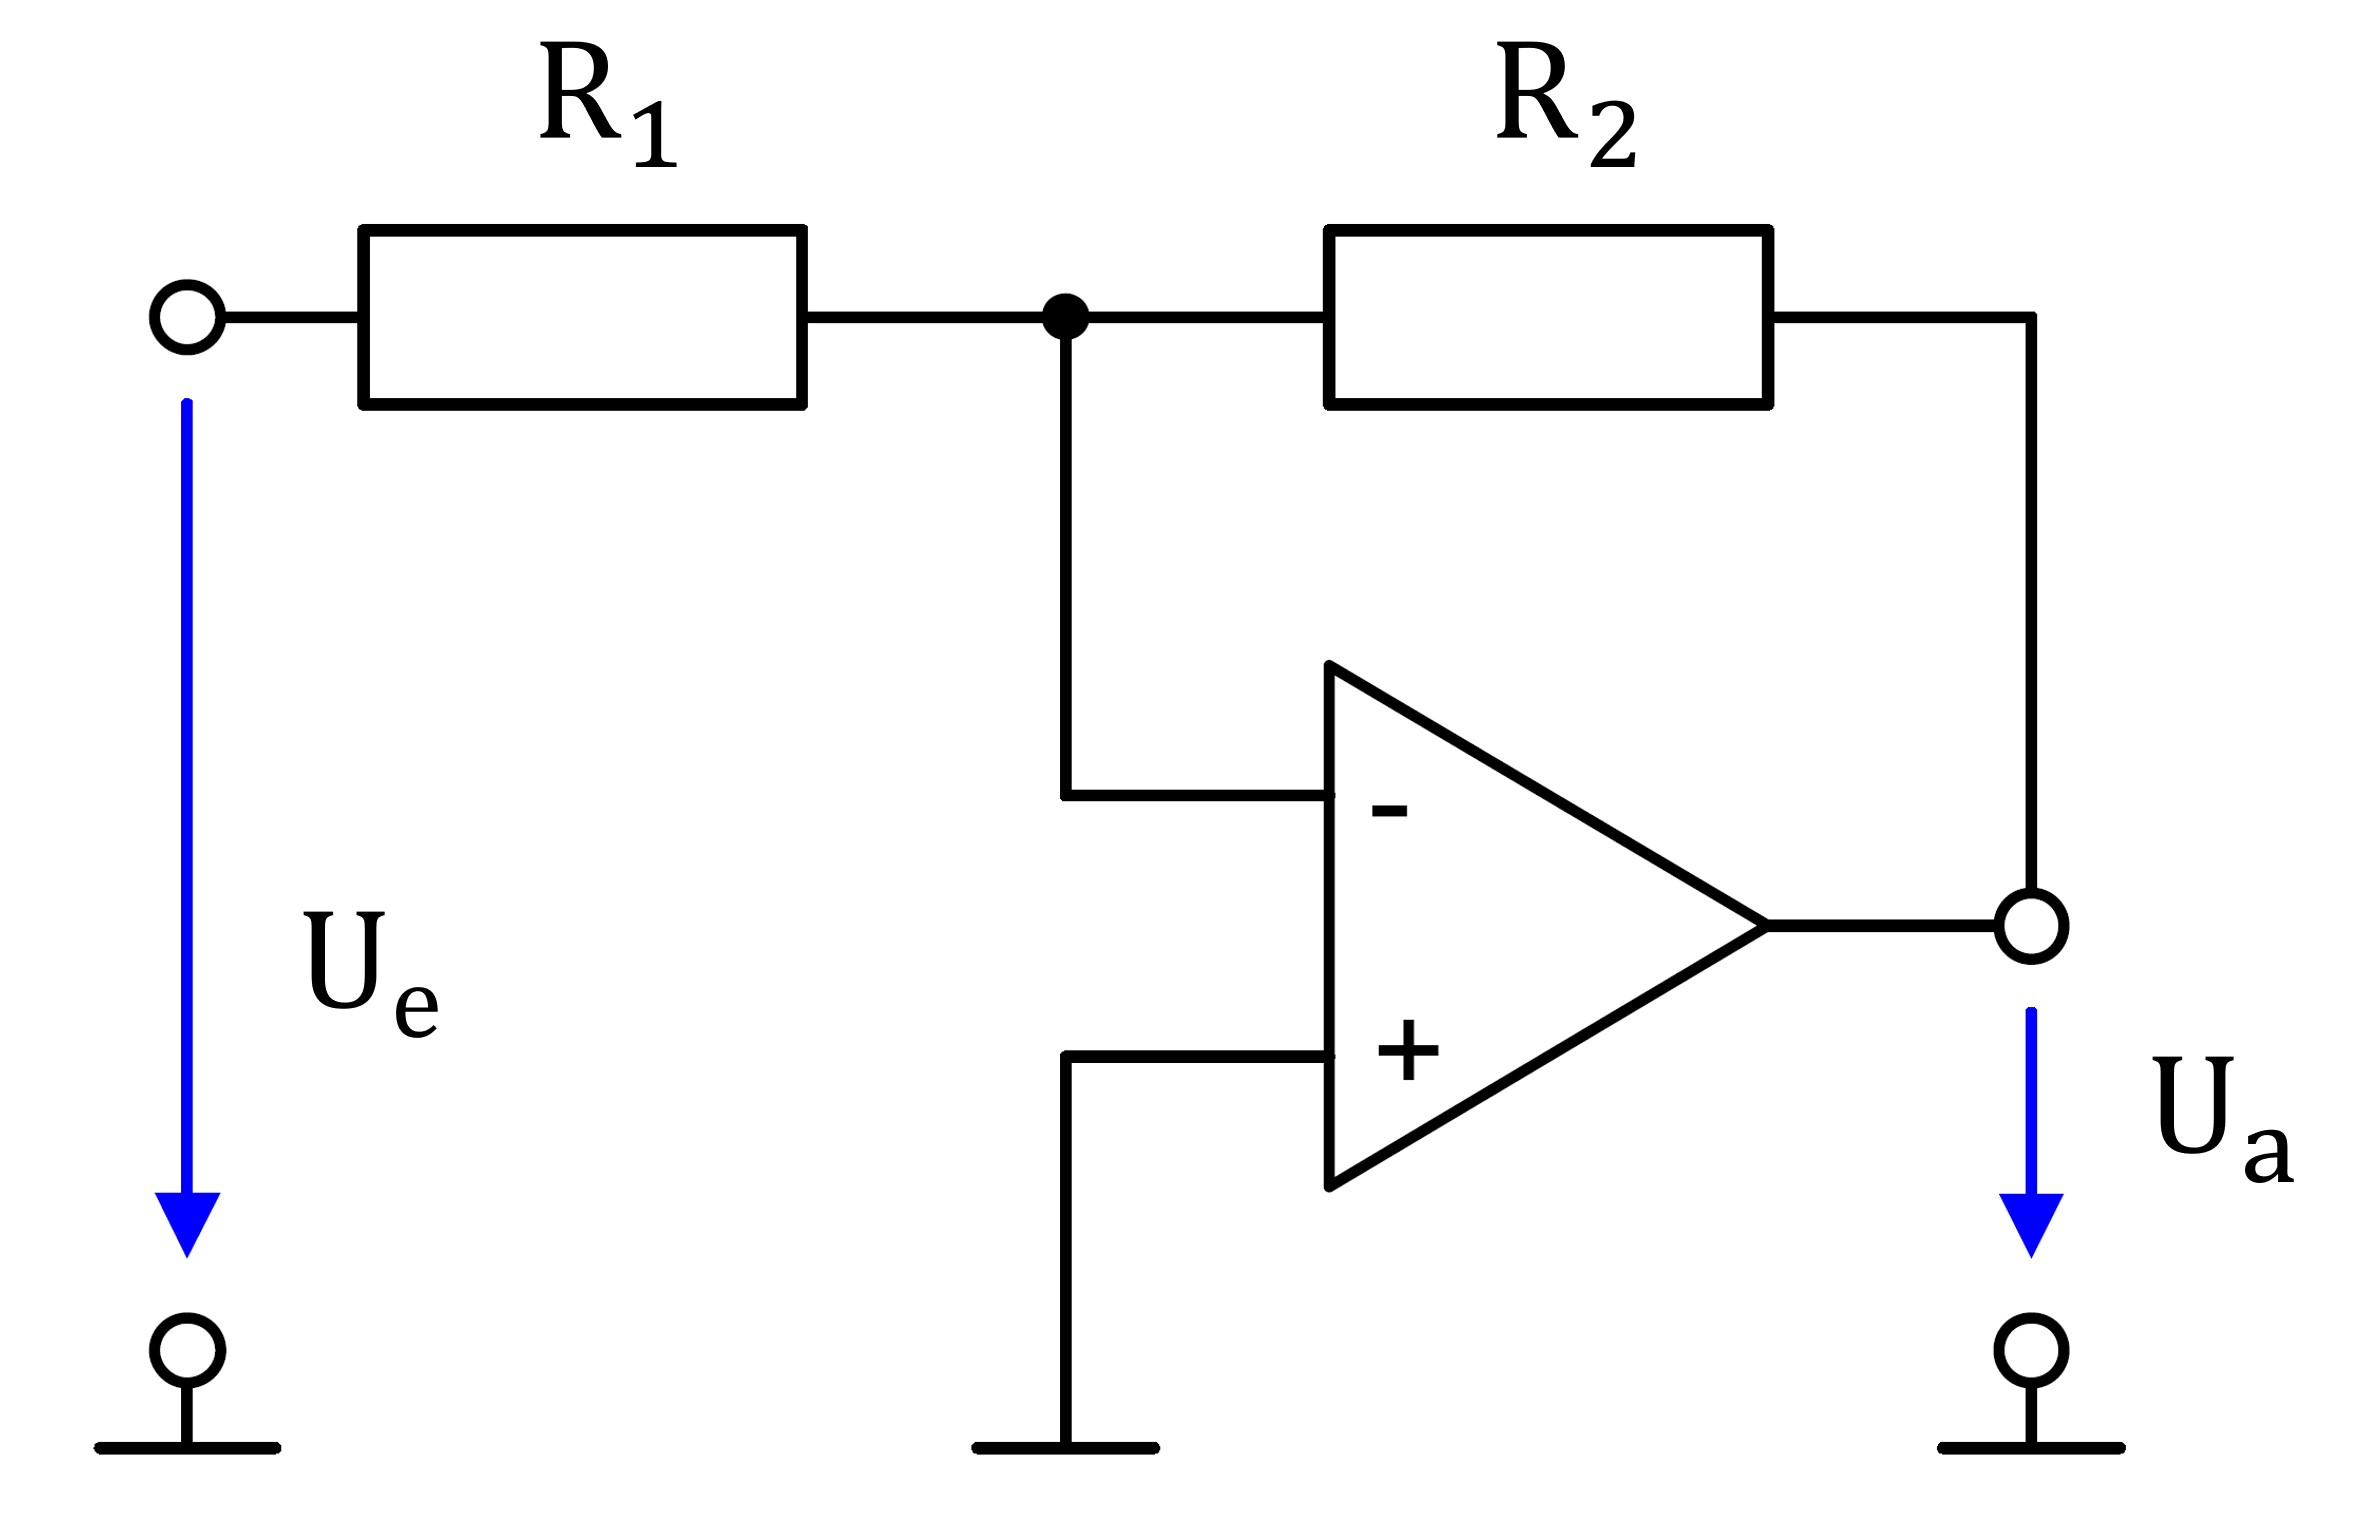
\includegraphics[width=0.7 \textwidth]{invOP.jpg}
	\caption[Invertierender Operationsverstärker]{Invertierender Operationsverstärker} 
	\gls{online:Eigen}
	\label{fig:ninvOP}
\end{figure}

Abbildung ~\ref{fig:ninvOP} zeigt die klassische Schaltung eines invertierenden Operationsverstärkers mit
Rückkopplungszweig. Dieser definiert über den Widerstand $R_{2}$ die Schleifenverstärkung, indem auf den invertierten Eingang ein Teil des Ausgangssignals zurückgeführt wird.  Bei einem steigenden Ausgangssignal wird so dem steigenden Eingangssignal entgegengewirkt. Dies gewährleistet, dass das Ausgangssignal nicht unendlich verstärkt werden kann. Der invertierende Eingang wird mit Masse verbunden. Zuletzt wird hier die Spannungsverstärkung $A$ der invertierenden Grundschaltung über den Rückkopplungspfad bestimmt. Diese ergibt sich hier also zu: 

\begin{equation}
	\label{equ:bsp1}
	A = - \frac{R_{2}}{R_{1}}
\end{equation}

und das negative Vorzeichen bedeutet, dass hier eine Phasendrehung des Signals um 180$\circ$ stattgefunden hat. Der invertierende Verstärker besitzt zudem die Fähigkeit Signale zu dämpfen. Daher wird er häufig für Filterschaltungen und messtechnische Zwecke benutzt. 

Die folgende Abbildung ~\ref{fig:ninvOP} illustriert den nicht-invertierenden Operationsverstärker in seiner Grundschaltung. Die Spannungsverstärkung berechnet sich anhand der Spannungsteiler Beziehung

\begin{equation}
	\label{equ:bsp1}
	U_{a} = U_{e} \cdot \frac{R_{1} + R_{2}}{R_{1}} = U_{e} \cdot (1+ \frac{R_{2}}{R_{1}})
\end{equation}
daraus ergibt sich dann
\begin{equation}
	\label{equ:bsp1}
	A = \frac{U_{a}}{U_{e}} = 1+ \frac{R_{2}}{R_{1}}
\end{equation}
Wegen seines kleinen Ausgangs- und großen Eingangswiderstandes eignet sich diese \gls{acr:OP}-Schaltung sehr gut als  Wechselspannungsverstärker und Impedanzwandler. Die Übertagungskennlinie ist in Abbildung ~\ref{fig:aussteuer} dargestellt. 

\begin{figure}[H]
	\centering
	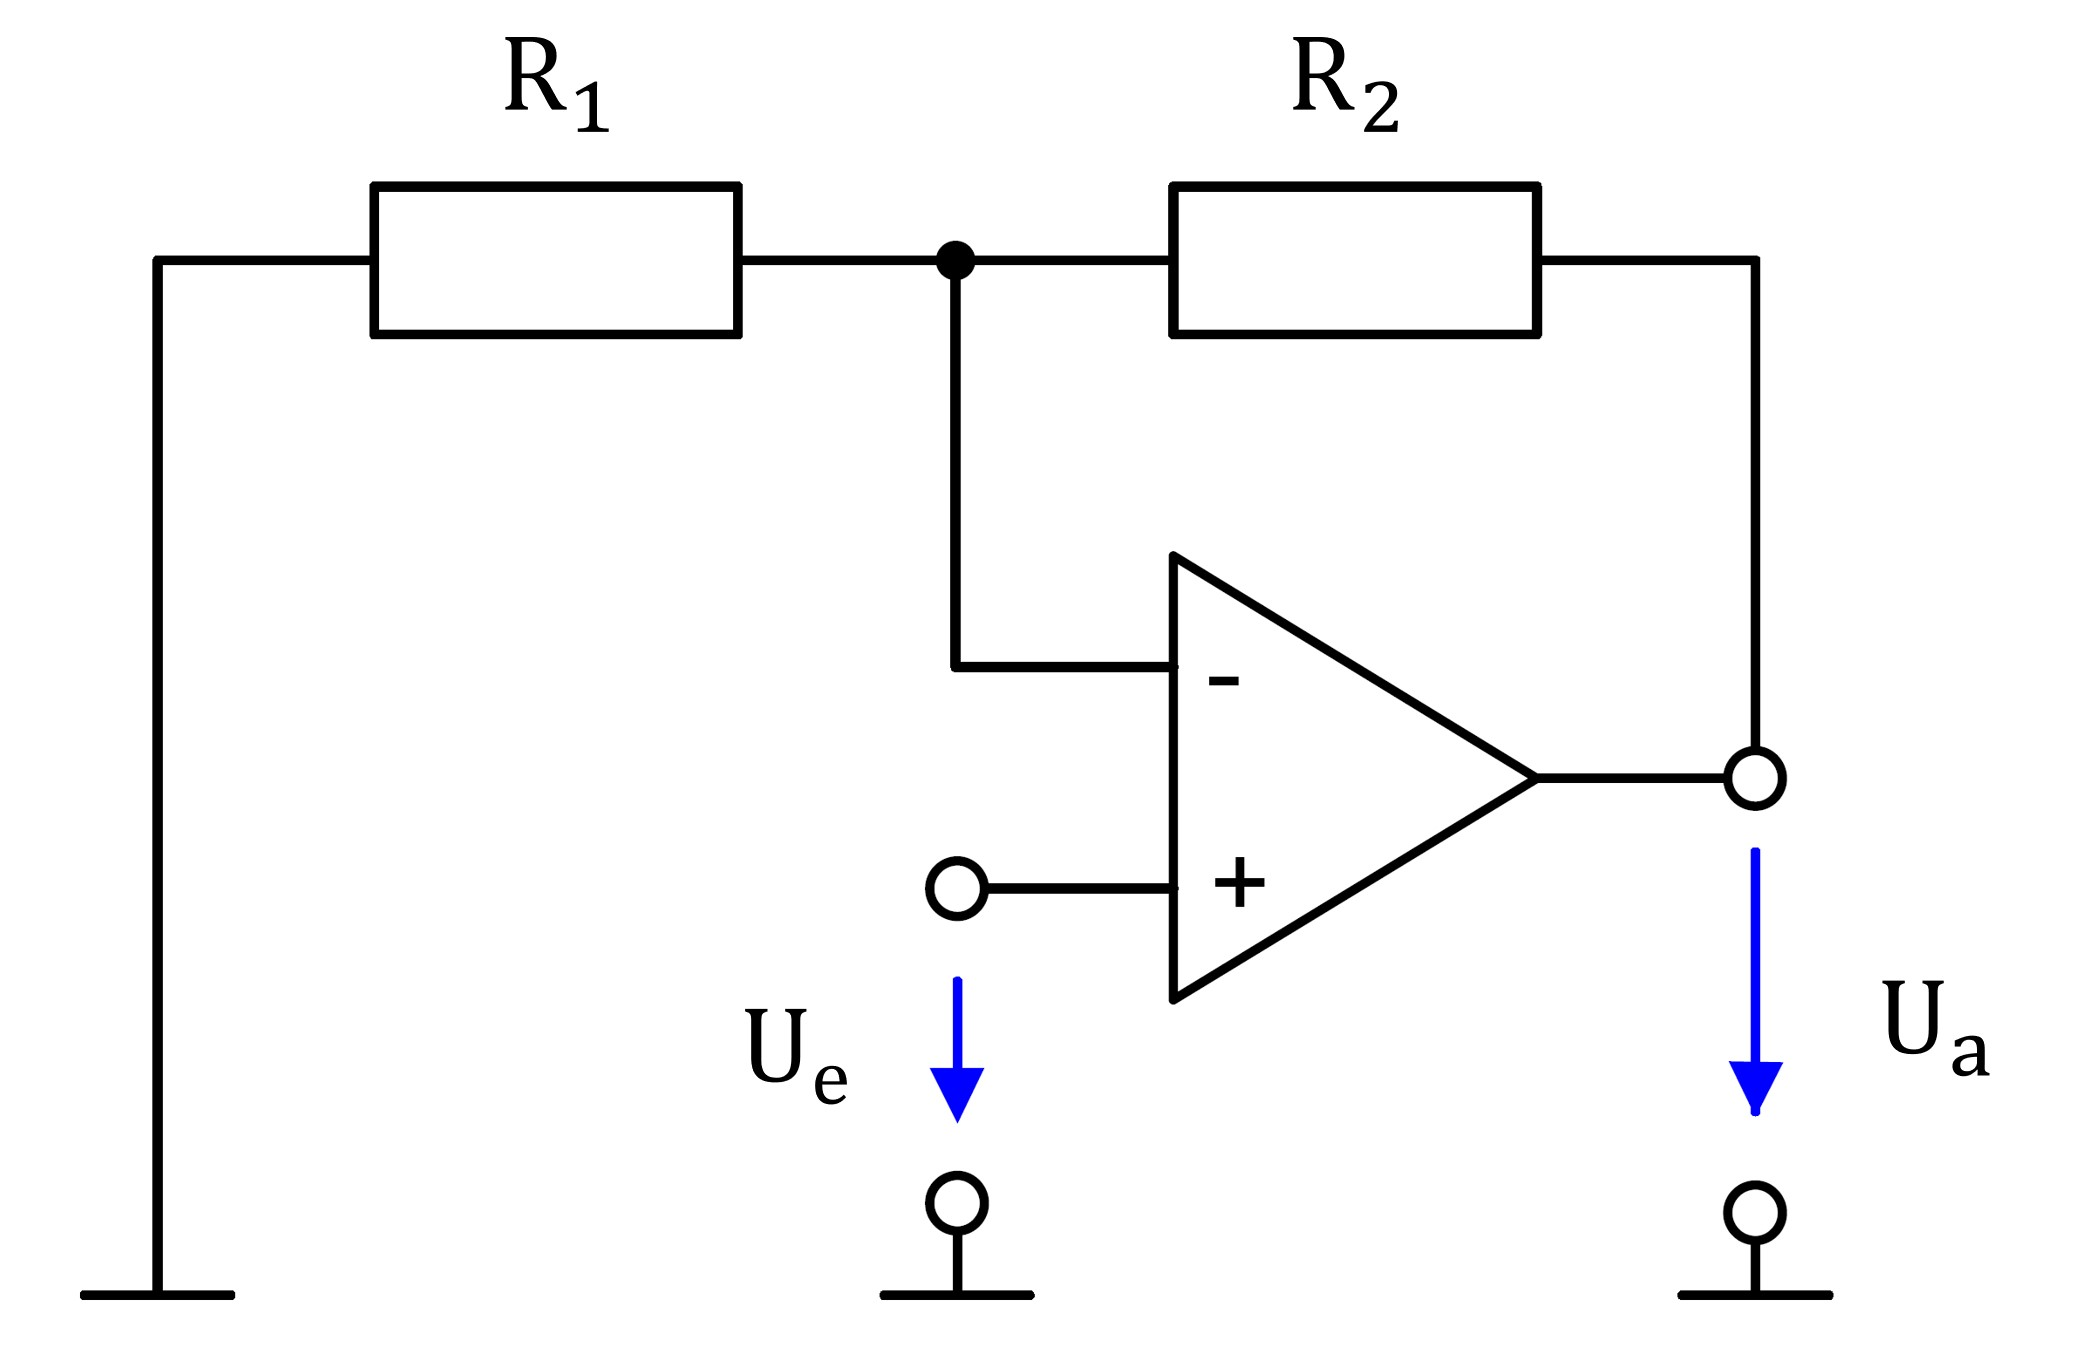
\includegraphics[width=0.7 \textwidth]{ninvOP.jpg}
	\caption[Nichtinvertierender Operationsverstärker]{Nichtinvertierender Operationsverstärker} 
	\gls{online:Eigen}
	\label{fig:invOP}
\end{figure}

Es zeigt auch die maximale Aussteuerbarkeit am Ausgang der \gls{acr:OP}s, welche innerhalb $V-$ < $U_{a}$ < $V+$ liegt. Werden entweder positive oder negative Grenzen erreicht, kann $U_{a}$ nicht weiter ansteigen. Dieser Zustand nennt sich Übersteuerung. Die klassischen Aussteuergrenzen liegen in etwa 1V unter der Versorgungsspannung.\cite{OP}

\begin{figure}[H]
	\centering
	\includegraphics[width=0.85 \textwidth]{aussteuer.jpg}
	\caption[Operationsverstärker]{Operationsverstärker} 
	\gls{online:Eigen}
	\label{fig:aussteuer}
\end{figure} 

\newpage
\subsection{Feldeffekttransistor}
\label{subsec:Unterabschnitt12}
Die am häufigsten eingesetzten Leistungsschutzschalter im Spannungsbereich von bis etwa 250V sind \gls{acr:MOSFET}.\gls{online:mosfet}


Sie sind eine Sonderform der Transistoren, welche auch unipolare Transistoren genannt werden. Sie besitzen einen Kanal aus Halbleitermaterial, auf dem horizontal zur Stromrichtung ein elektrisches Feld entsteht, welches den Querschnitt des Kanals verändert. Damit wird der Stromfluss durch das Bauteil geregelt. Im Field-Effect Transistor (FET) steuert eine Spannung den Strom. Es gibt vier Grundbauformen von \gls{acr:MOSFET}. Einen \gls{acr:NMOS} und einen \gls{acr:PMOS} Typus und davon jeweils eine selbstsperrende und eine selbstleitende Variante. Im Anwendungsfall dieser Thesis wird ein \gls{acr:NMOS} verwendet. \cite{heringElektrotechnikUndElektronik2018}

\newpage
\subsection{Digital Potentiometer}
\label{subsec:Unterabschnitt12}

Um den Strom durch die \gls{acr:LED} digital zu regulieren und demgemäß die Helligkeit der \gls{acr:LED} für die Datenübertragung zu variieren, wird ein Digitalpotentiometer benötigt. Hierfür wurde der \gls{acr:IC} MCP42010 in der 10k$\ohm$–Variante mit 2 Kanälen ausgewählt. Dieses Digitalpotentiometer kann über ein \gls{acr:SPI} mittels eines Arduino angesteuert werden, um dessen Widerstandswert in 256 Schritten zu verändern. Dies ermöglicht eine Variation des Widerstandes in einem Bereich zwischen 52$\ohm$ (00h) und 10k$\ohm$ (FFh) in 39$\ohm$ Schritten. 
Die vom \gls{acr:IC} vorgeschriebene Versorgungsspannung von 5V stellt der Spannungsversorgungspin des Arduino bereit. Außerdem kann dem Datenblatt des \gls{acr:IC}s die Information entnommen werden, dass dessen Eingangsspannungsbereich an den Widerstandseingängen maximal zwischen -0.5V und 6V liegen darf. Da der IC in dieser Schaltung mit 5V betrieben wird, dürfen die Widerstandseingänge mit einer Spannung von maximal -0.6V bis 6V belastet werden. Das ist ein äußerst wichtiges Kriterium für die Auslegung der Schaltung, da hier über die Grenzen der maximalen Amplitude entschieden werden muss, um unerwünschten Nebeneffekten vorzubeugen.

\begin{figure}[H]
	\centering
	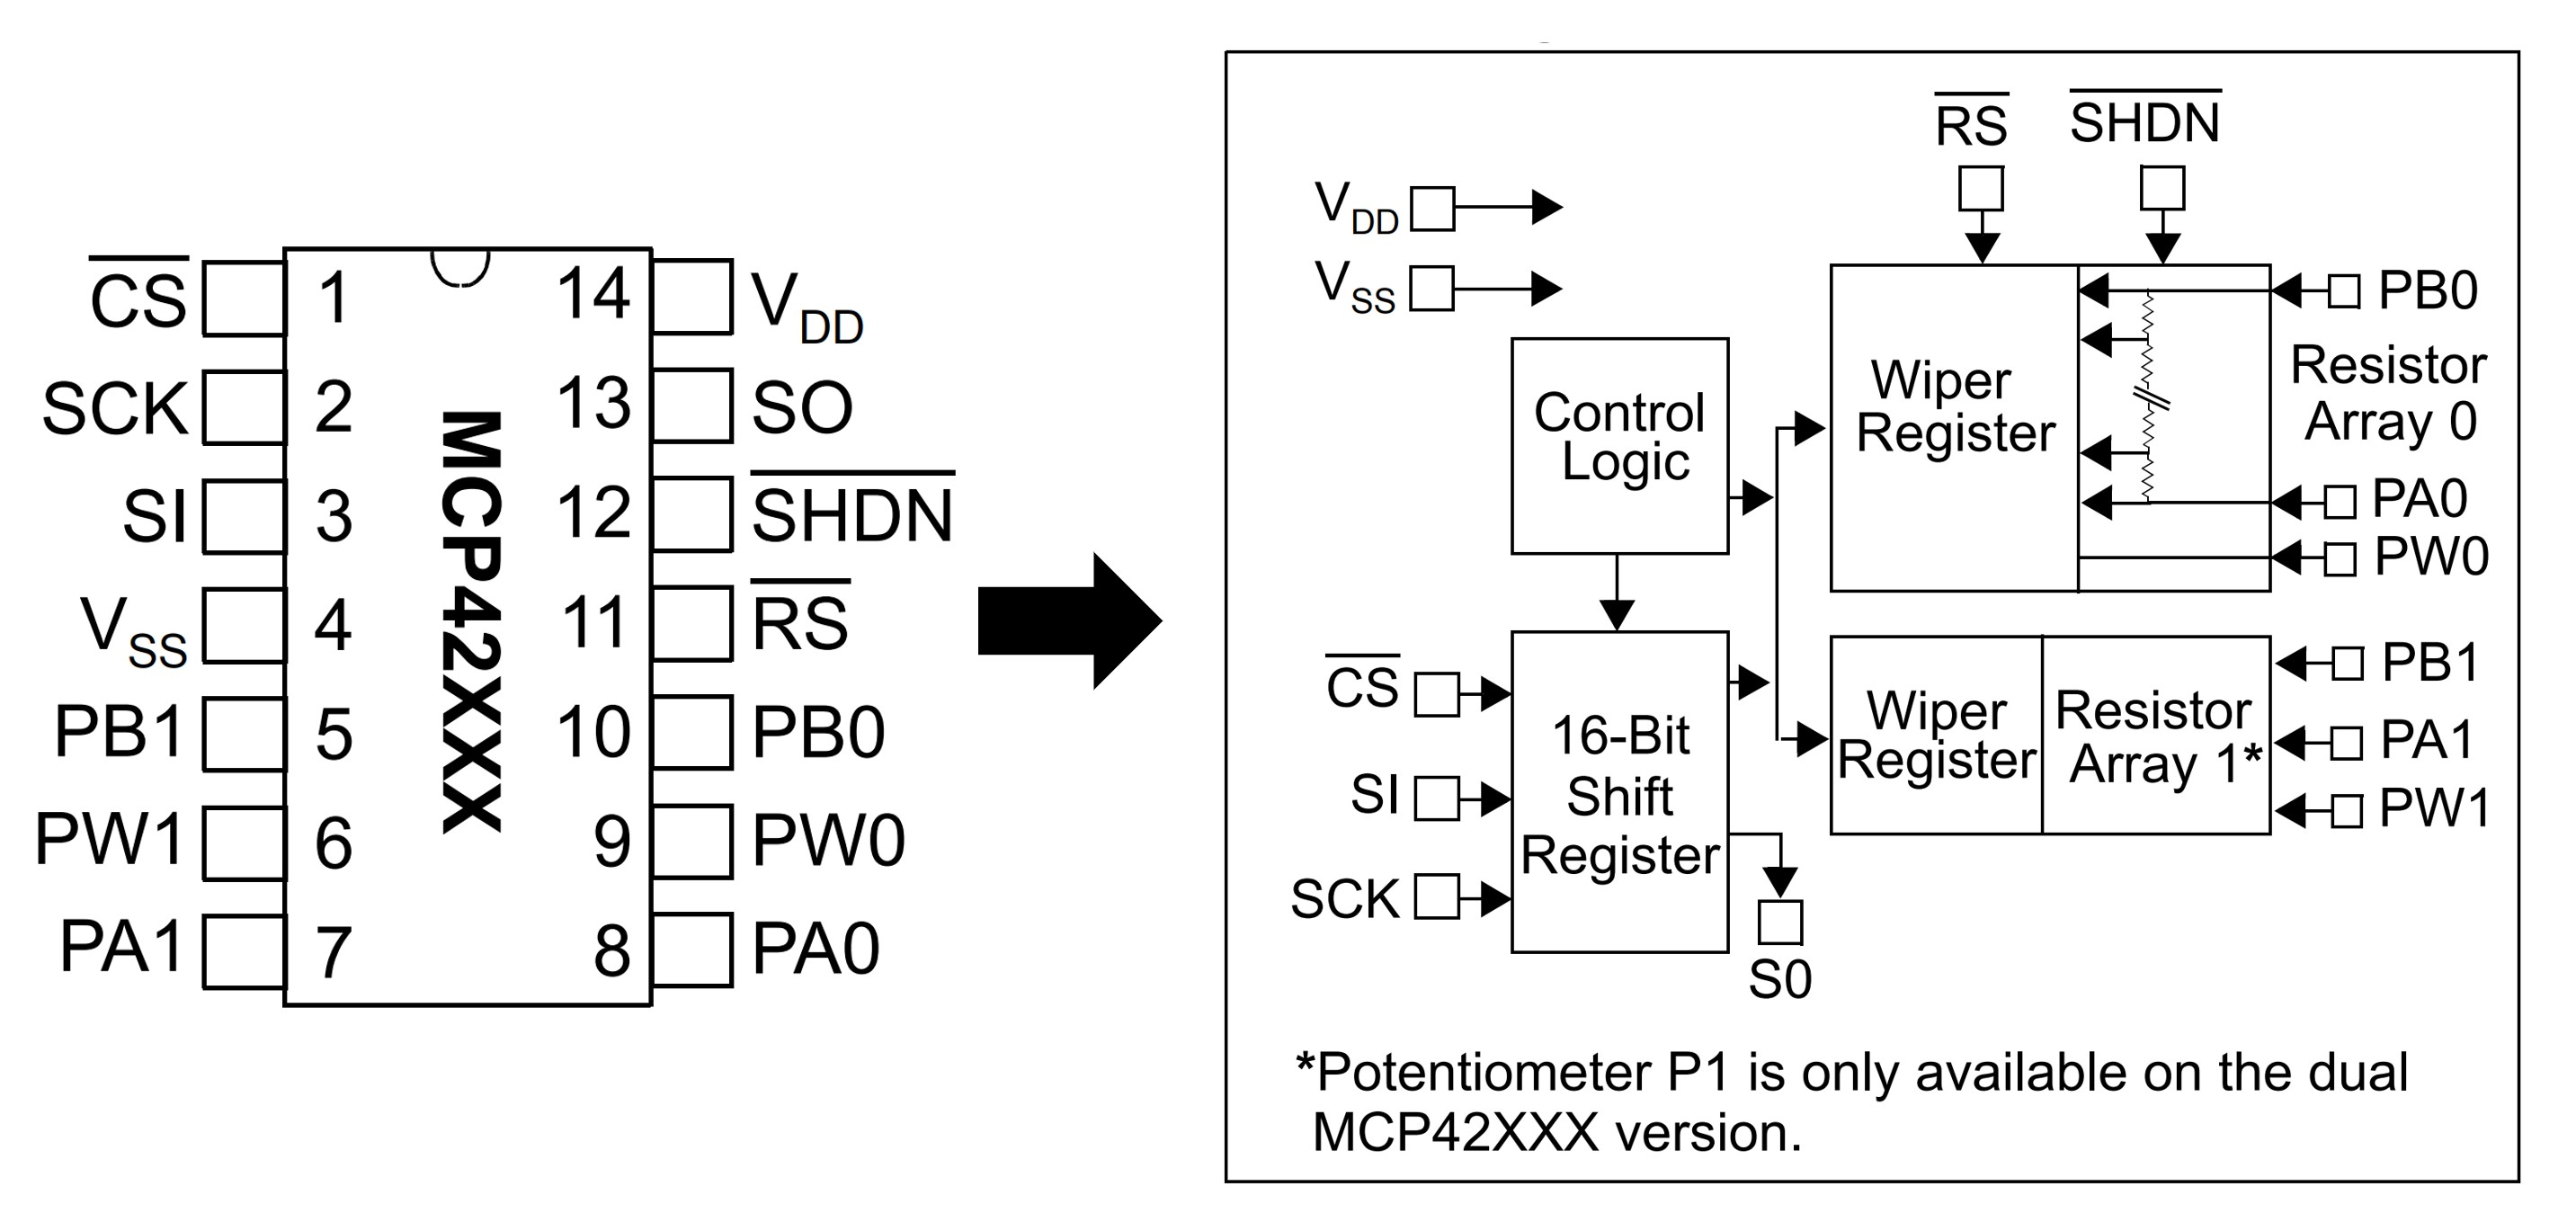
\includegraphics[width=0.8 \textwidth]{MCP.jpg}
	\caption[Aufbau des MCP42010]{Aufbau des MCP42010} 
	\cite{MCP42}
	\label{fig:MCP}
\end{figure}

Die Funktion der einzelnen Pins und wie man den \gls{acr:IC} mit dem Arduino verbindet, wird in nachfolgender Tabelle~\ref{tab:pinmcp} beschrieben. 
\begin{table}[htb]
	\begin{center}
		\begin{tabular}[H]{cccc}	
			\toprule
			\textbf{Pin Nr.} & \textbf{Name}  &\textbf{Funktion} & \textbf{Arduino Pin Nr.} \\
			\midrule
			1 & $\overline{CS}$ & Chip Select &  10 \\
			2 & SCK & Serial Clock &  13 \\
			3 & SI & Serial Data Input&  11 \\
			4 & $V_{SS}$ & Ground &  Ground \\
			5 & PB1 & Terminal B Connection For Pot 1 & X \\
			6 & PW1 & Wiper Connection For Pot 1 &  OP-1 Minus \\
			7 & PA1& Terminal A Connection For Pot 1 &  OP-1 Out  \\
			8 & PA0& Terminal A Connection For Pot 0 &  5V \\
			9 & PW0& Wiper Connection For Pot 0 & OP-2 Offset \\
			10 & PB0 & Terminal B Connection For Pot 0 &  Ground \\
			11 & $\overline{RS}$ & Reset Input & X  \\
			12 & $\overline{SHDN}$ & Shutdown Input &X\\
			13 & SO & Data Out for Daisy-Chaining & X \\
			14 & $V_{DD}$ & Power & 5V \\
			\bottomrule
		\end{tabular}
		\caption{Anschlussinformation und Pinbelegung des MCP42010}
		\label{tab:pinmcp}
	\end{center}
\end{table}
Aufgrund des Anwendungsfalls in dieser Thesis, werden Pin 11 und Pin 12 des MCP42010 nicht benötigt und aus diesem Grund nicht am Arduino angeschlossen. 

\subsection{DC/DC Spannungswandler}
\label{subsec:Unterabschnitt12}

Ein Gleichspannungswandler, oder auch DC-DC-Wandler, wandelt eine der Schaltung zugeführte Eingangsgleichspannung in eine geregelte Ausgangsgleichspannung, welche ein anderes Spannungsniveau als die Eingangsspannung aufweist. Diese kann beispielsweise niedriger, höher oder auch invertiert sein.
Da die zu übertragenden Daten am Ausgang der Soundkarte als reine Wechselspannung anliegen, wird eine negative Spannungsquelle für die vorhandenen Operationsverstärker benötigt, um kein Risiko auf Datenverluste einzugehen.
Gleichspannungswandler werden grundsätzlich immer dort eingesetzt, wo die zu Verfügung stehende Eingangsspannung nicht zur Versorgung der im Schaltkreis folgenden elektronischen Bauteile passt.[AbcderPowerModuleGrundlagen.pdf] Aufgrund der Unkonventionalität, sowohl eine negative als auch eine positive Spannungsquelle simultan an die Platine anzuschließen, wandelt der DC/DC-Spannungswandler diese negative Spannung direkt auf der Platine um. Der LT1054 wird auch ”negative voltage generator” genannt. Das ist ein Bauteil, welches eine negative Ausgangsspannung erzeugt. Diese ist proportional zur Eingangsspannung $V_{CC}$. Zum Nutzen dieses Bauteils als einfachen DC-DC-Wandler mit invertierender Funktion muss es laut Datenblatt an den Ausgängen mit zusätzlichen Kondensatoren beschalten werden. Aufgrund dessen, dass der DC-DC-Wandler mit negativen Spannungen arbeitet, ist es signifikant, im Falle der Nutzung von Elektrolytkondensatoren, auf die Polung der Kondensatoren zu achten. Jene sind unidirektional, was in Abbildung~\ref{fig:DCDC} illustriert ist. Zusätzlich ist zu erkennen, dass am negativen Ausgang des DC-DC-Wandlers nicht genau -12V anliegen sondern etwa -11.35V. Dies ist auf den Wirkungsgrad des DC-DC-Wandlers zurückzuführen und ist unter - Voltage Loss - im Datenblatt zu finden. 

\begin{figure}[H]
	\centering
	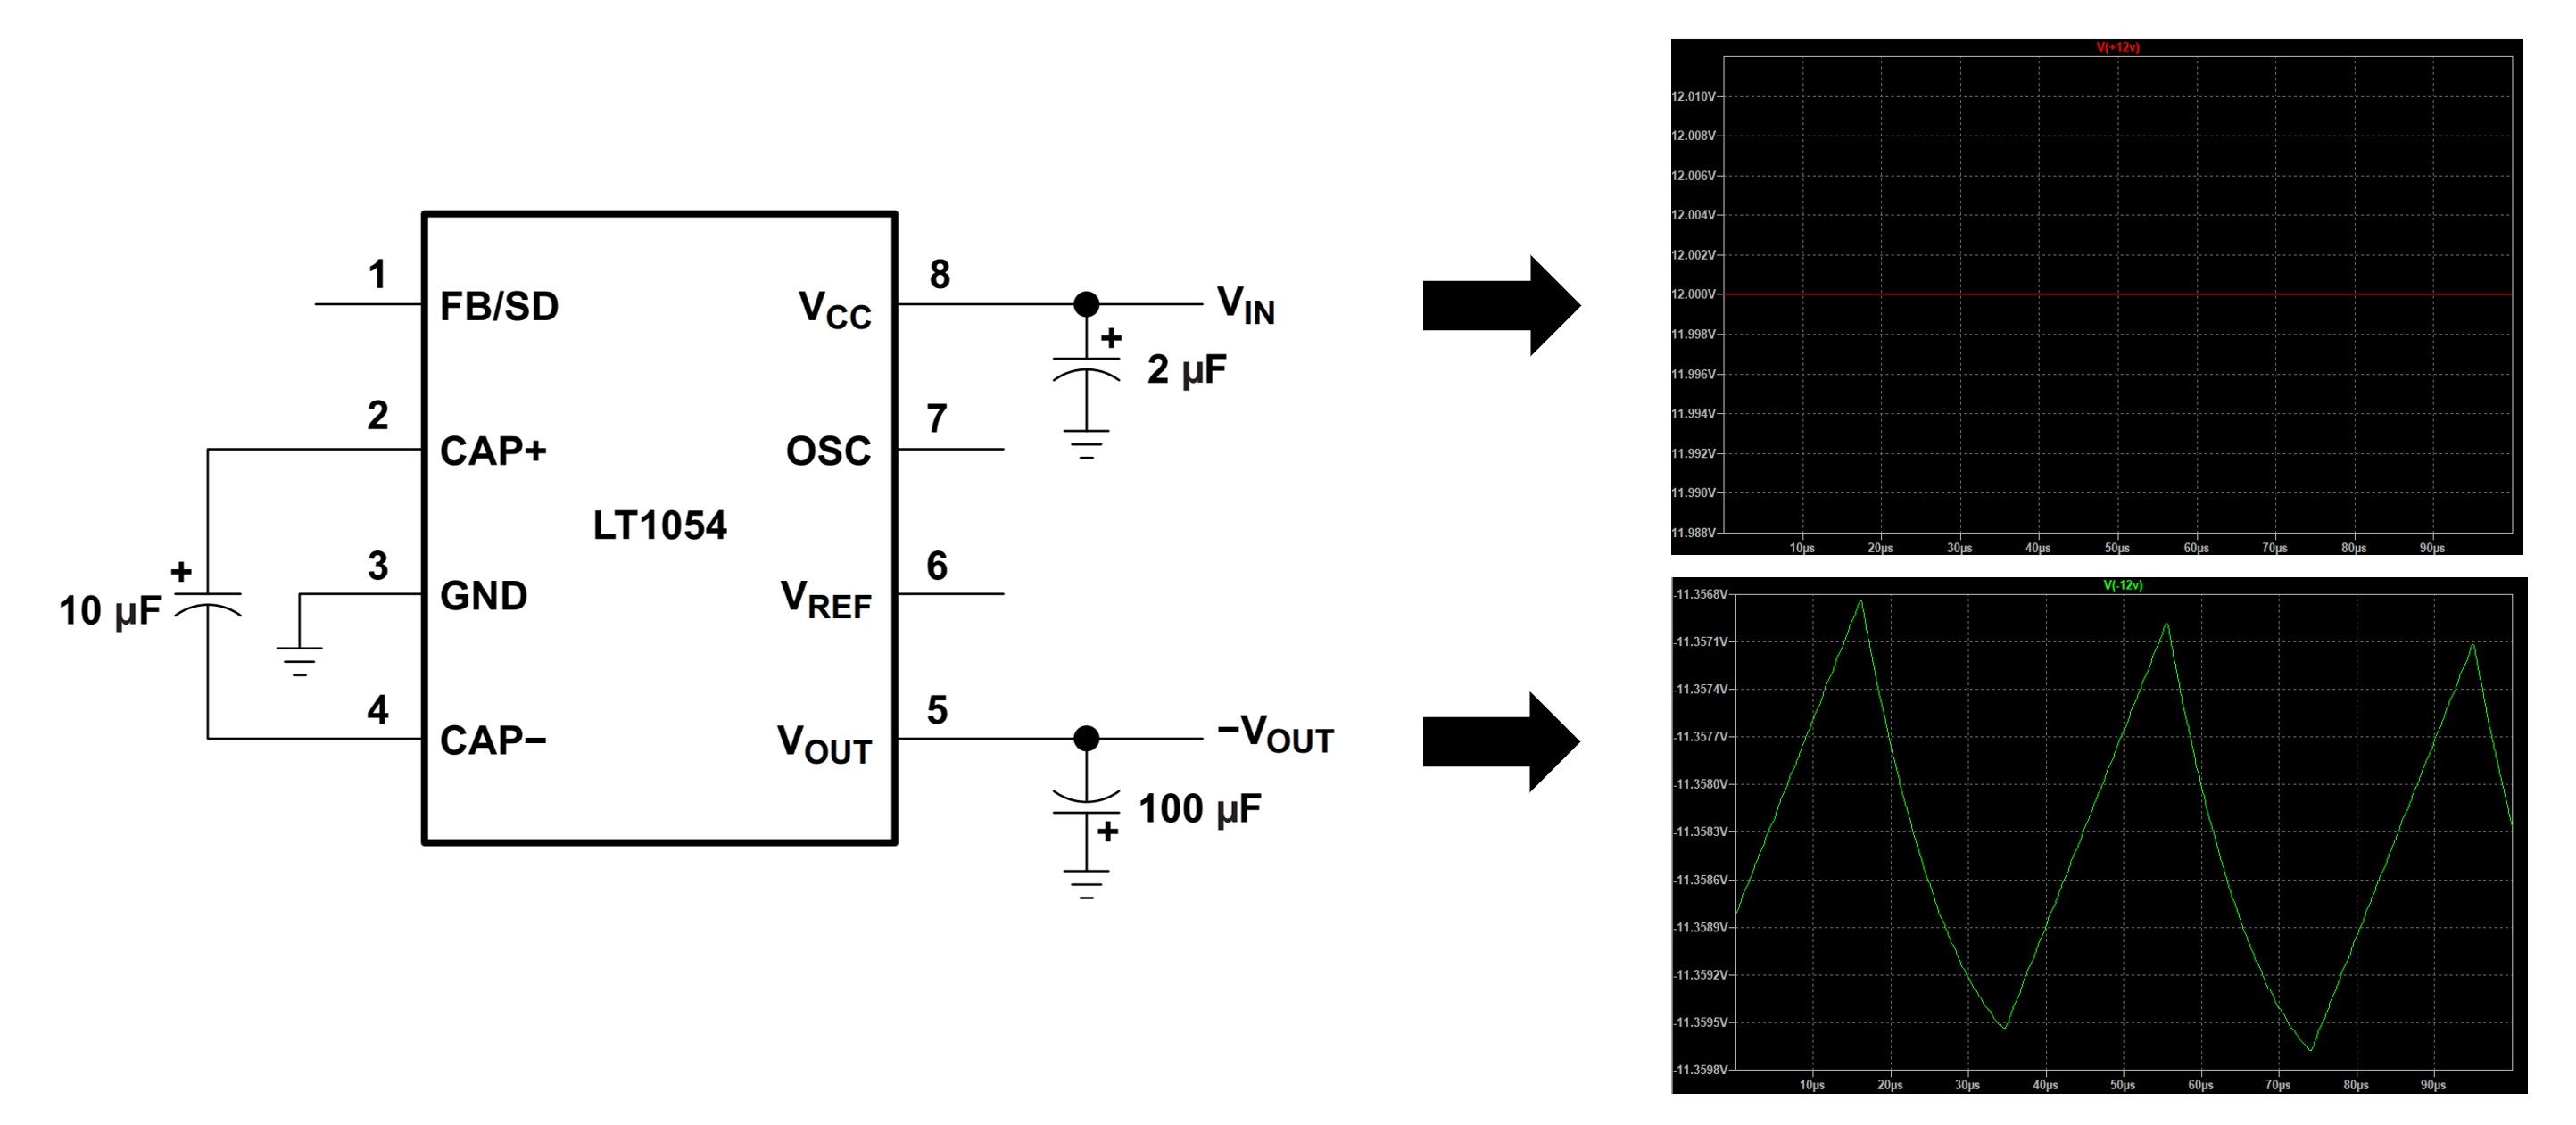
\includegraphics[width=0.6 \textwidth]{DCDC.jpg}
	\caption[Beschaltung und erzeugte Spannung des LT1054]{Beschaltung und erzeugte Spannung des LT1054} 
	\gls{online:Eigen}+Datenblatt
	\label{fig:DCDC}
\end{figure}

Der Spannungswandler arbeitet außerdem intern für die Invertierung mit einer Nennfrequenz von 25kHz. Da die zu übertragenden Daten auch nahe diesem Bereich liegen, empfiehlt es sich, den Pfad der Signalverarbeitung und den der Spannungsinvertierung auf der Platine möglichst weit auseinander zu platzieren, um möglichen parasitären Störungen vorzubeugen.


\subsection{Arduino UNO V3}
\label{subsec:Unterabschnitt12}

Die Arduino-Plattform besteht prinzipiell aus der auf C und C++ basierenden Entwicklungsumgebung und der zu programmierenden Hardware\gls{online:arduino}. Vorteilhaft ist hier die gute Dokumentation und eine große Menge an Bibliotheken zum Einbinden externer Hardwarekomponenten. Ein zusätzlicher Vorteil der Plattform liegt in ihrer Quelloffenheit. Alle zugehörigen Komponenten sind demnach 'Open Source'. Das hat zur Folge, dass Codes der Bibliotheken und des Bootloaders frei zur Verfügung stehen und nach Belieben verändert werden können. Auch die Architektur der Hardware ist offengelegt, weshalb Hersteller eigene kompatible Boards konstruieren und verkaufen können. Durch die Unabhängigkeit von Programmierer und Hersteller entsteht eine erschwingliche Hardware, welche bezüglich der Quelloffenheit ohne Einschränkungen programmiert werden kann.[10 - Evans, Beginning Arduino Programming. Apress, 2011, ISBN: 978-1-4302-3777-8]Diese eignet sich hervorragend zur Funktionsprogrammierung von ansteuerbaren Komponenten im analogen Signalverarbeitungspfad.

\section{Tools}       
\subsection{LT-Spice}
\label{subsec:Unterabschnitt12}
LT-Spice ist eine SPICE-basierte Computersoftware zur Simulation analoger, elektronischer Schaltungen. Diese wurde vom Halbleiterhersteller Analog Devices (ursprünglich von Linear Technology) entwickelt. Es ist die am weitesten verbreitete und verwendete SPICE-Software in der Elektro-Simulationsbranche. Obwohl es sich um freie Software handelt, ist LT-Spice nicht künstlich eingeschränkt, um seine Funktionalität einzuschränken.\gls{online:spice} Diese Simulationssoftware wurde im Rahmen dieser Arbeit zur Erprobung und Simulation des analogen Signalverarbeitungsschaltkreises verwendet.

\subsection{Eagle}
\label{subsec:Unterabschnitt12}

EAGLE ist eine Software zum Designen und Erstellen von Leiterplattenlayouts. Die Software verfügt über einen Schaltplan- und einen Layouteditor, sowie über eine sehr umfassende Bibliothek an Bauteilen, welche sehr unkompliziert und individuell erweiterbar ist.\gls{online:eagle1}\gls{online:eagle2}

Signifikant für die Dimensionierung des Platinenlayouts ist Tabelle~\ref{tab:leiterbahnen}. Hier werden die verschieden Leiterbahnbreiten und Leiterbahnabstände dargestellt, welche für ein funktionierendes Platinenlayout unabdingbar sind.

\begin{table}[htb]
	\begin{center}
		\begin{tabular}[h]{cccc}	
			\toprule
			Spannung [V] & Max. Strombelastung [A]& Leiterbahnbreite [mil] & Leiterbahnabstand[mil] \\
			\midrule
			5 & 0.6&6 & 8 \\
			10 & 0.8&8 & 13 \\
			30 & 2.0&20& 30\\
			150 &2.7&30 & 50 \\
			230& 3.5&50 & 100 \\
		\bottomrule
		\end{tabular}
		\caption{Richtlinien zu Leiterbahnbreite und Leiterbahnabständen}
		\label{tab:leiterbahnen}
	\end{center}
\end{table}

\subsection{Arduino IDE}
\label{subsec:Unterabschnitt12}

Die Sprachen, welche in der Entwicklungsumgebung genutzt werden sind C und in kleineren Umfängen auch C++. In den Standardbibliotheken der Entwicklungsumgebung sind die für die Programmierung erheblichsten Funktionen zusammengefasst. Um weitere Funktionen zu nutzen, können dementsprechend zusätzliche Bibliotheken eingebunden werden. 
Der Editor mit integriertem Compiler ist ein weiterer Bestandteil des \gls{acr:IDE}. In diesem wird der Code geschrieben, kompiliert und auf das Board überspielt. User benötigen also nur eine Software, um ihre Mikrocontroller in vollen Umfängen nutzen zu können. Dieses \gls{acr:IDE} bietet außerdem die Möglichkeit, Bibliotheken oder gar Programmbeispiele herunterzuladen. 

[10B. Evans, Beginning Arduino Programming. Apress, 2011, ISBN: 978-1-4302-
3777-8.].

\begin{figure}[H]
	\centering
	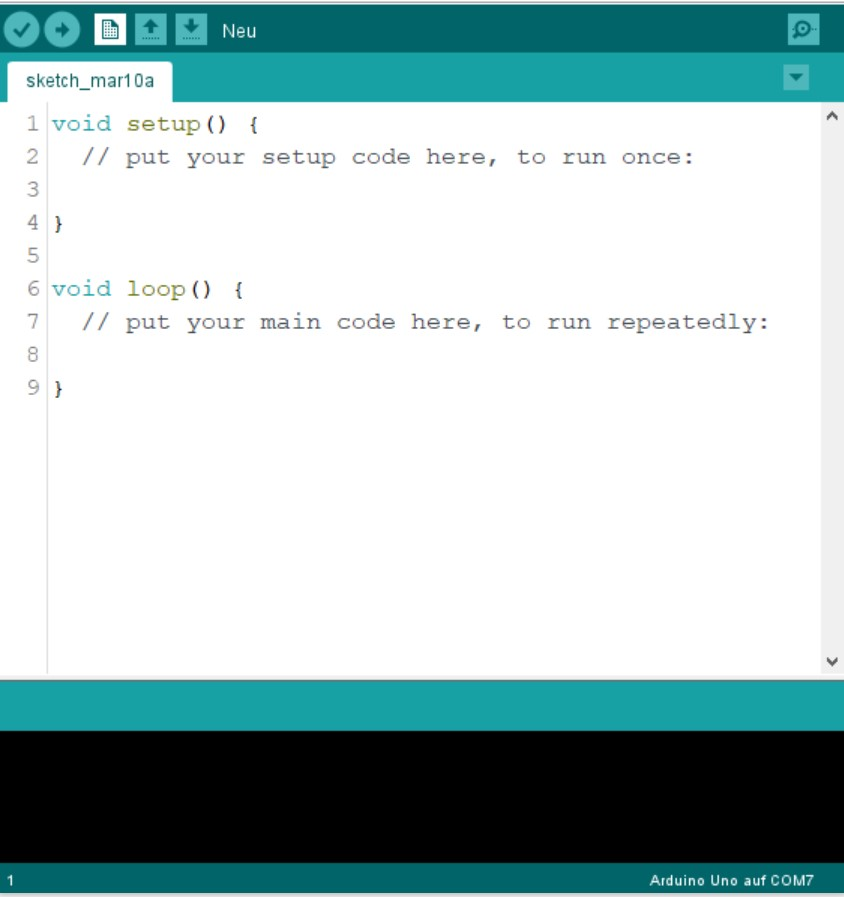
\includegraphics[width = 0.6 \textwidth ]{ide.jpg}
	\caption[Arduino \gls{acr:IDE}]{Arduino \gls{acr:IDE}}\gls{online:Eigen}
	\label{fig:ide}
\end{figure}


Arduino-Programme basieren immer auf einem einheitlichen Grundaufbau. In Abb. ist
dieser zu erkennen. Es sind zwei Funktionen namens setup() und loop() deklariert.
Setup() wird einmalig zu beginn des Programms aufgerufen, während loop() direkt im Anschuss aufgerufen wird, bis der Mikrocontroller stromlos geschaltet wird. Oberhalb der Funktion setup() können außerdem noch Präprozessorbefehle programmiert werden.

\subsection{Dream}
\label{subsec:Unterabschnitt12}
Die Software Dream bietet eine Alternative um Radiosignale auf dem Computer zu empfangen und auch zu senden. Sie war ursprünglich als Forschungsprojekt des Fraunhofer Instituts angesetzt. Signale, welche nicht über den PC empfangen werden können, werden über den Mikrofoneingang der Soundkarte empfangen.
Bei alldem benutzt das Konzept internationale Direktiven für Amateurfunk, Radio und Informationsdienste.
Diese Eigenschaft ermöglicht es dem User, FM, AM und \gls{acr:DRM} zu empfangen. Außerdem visualisiert die Software in Echtzeit zahlreiche Daten, Statistiken und Diagramme des empfangenen Signals. \gls{online:dream} Die Modulation und das Senden des OFDM-Signals über die konstruierte Hardware erfolgt durch diese Software und wird in den folgenden Kapiteln noch weiter intensiviert.